\documentclass[aspectratio=169,9pt]{beamer}
\graphicspath{{figures/}} % Setting the graphicspath

% Theme settings
\usetheme{Madrid}
\usecolortheme{default}
\setbeamertemplate{navigation symbols}{}   % removes navigation symbols such as 'next page'
\setbeamertemplate{footline}{}             % remove line with name, date, page nr. 
\setbeamercolor*{frametitle}{bg=white}     % remove background from frametitle
\usepackage{caption}
% \captionsetup[figure]{labelformat=empty}% redefines the caption setup of the figures environment in the beamer class.
\setbeamersize{text margin left=20pt,text margin right=10pt}

\usefonttheme[onlymath]{serif} % makes beamer math look like article math


%======================= import packages =======================================
\usepackage{pifont}       % Pi fonts (Digbats, symbol, etc.)
\usepackage{graphicx}     % More options for \includegraphics
\usepackage{tikz}
\usepackage{appendixnumberbeamer} % separate appendix numbering
\usepackage{booktabs}
\usepackage{hyperref}
\usepackage{tabularx}
\usepackage{amsmath, nccmath}
\usepackage{xcolor}
\usepackage[absolute,overlay]{textpos} % for texblock




%======================= page numbering =======================
\addtobeamertemplate{navigation symbols}{}{ \usebeamerfont{footline}
  \insertframenumber / \inserttotalframenumber \hspace*{2mm} \\ \vspace*{1mm} 
}


%=================================== colors ====================================
\definecolor{RoyBlue}{RGB}{22, 46, 69}
\definecolor{RoyGrey}{RGB}{64, 88, 128} 

\newcommand{\hlme}[1]{{\color{red}\bf #1}} % highlight me

\setbeamercolor{structure}{fg=RoyBlue} % itemize, enumerate, etc
\setbeamercolor{frametitle}{fg=RoyGrey}
 \setbeamercolor{section in head/foot}{bg=RoyBlue}


%======================= add progress dots to headline =========================
\setbeamertemplate{headline}{%
    \begin{beamercolorbox}[ht=4mm,dp=4mm]{section in head/foot}
        \insertnavigation{\paperwidth}
    \end{beamercolorbox}%
}%
\makeatother


%======================= add section title page ================================
\AtBeginSection[]{
  \begin{frame}
  \vfill
  \centering
    \usebeamerfont{title}\insertsection\par%
  \vfill
  \end{frame}
}


%=================================== titlepage =================================
\title{The NNPDF4.0 global analysis of the proton structure}
\date{ICHEP 2022, 7 July 2022}
\author{Roy Stegeman}
\institute{University of Milan and INFN Milan}
\titlegraphic{\vspace*{6mm}
    
\includegraphics[height=0.8cm]{logos/LOGO-ERC.jpg} \hspace{10mm}
	
\includegraphics[height=0.8cm]{logos/n3pdflogo_noback.png} \hspace{10mm}
	
\includegraphics[height=0.6cm]{logos/nnpdf_logo_official.pdf} \hspace{10mm}
	\includegraphics[height=0.8cm]{logos/Logo_Università_degli_Studi_di_Milano(not_mandatory).png}
	
\includegraphics[height=0.8cm]{logos/INFN_logo.png}
    \vspace*{5mm} \\
	\centering{ 
	\fontsize{7.0pt}{0.0pt}\selectfont This project has received funding from the European Union’s Horizon 2020 \\	
    \vspace*{-1mm}
	research and innovation programme under grant agreement No 740006.
	}
}

\defbeamertemplate{title page}{noinstitute}[1][]
{
  \vbox{}
  \vfill
  \begingroup
    \centering
    \begin{beamercolorbox}[sep=8pt,center,#1]{title}
      \usebeamerfont{title}\inserttitle\par%
      \ifx\insertsubtitle\@empty%
      \else%
        \vskip0.25em%
        {\usebeamerfont{subtitle}\usebeamercolor[fg]{subtitle}\insertsubtitle\par}%
      \fi%     
    \end{beamercolorbox}%
    \vskip1em\par
    \begin{beamercolorbox}[sep=0pt,center,#1]{author}
      \usebeamerfont{author}\insertauthor
    \end{beamercolorbox}
	\begin{beamercolorbox}[sep=0pt,center,#1]{author}
		\usebeamerfont{institute}\insertinstitute
	\end{beamercolorbox}
	\vspace*{8pt}
	\begin{beamercolorbox}[sep=0pt,center,#1]{author}
		On behalf of the NNPDF Collaboration \\
        {\small \href{https://arxiv.org/abs/2109.02653}{Eur.Phys.J.C 82 (2022) 5, 428;\quad arXiv:2109.02653}}
	\end{beamercolorbox}
	\vspace*{16pt}
    \begin{beamercolorbox}[sep=0pt,center,#1]{date}
      \usebeamerfont{date}\insertdate
    \end{beamercolorbox}\vskip0.5em
    {\usebeamercolor[fg]{titlegraphic}\inserttitlegraphic\par}
  \endgroup
  \vfill
}

\makeatletter
\setbeamertemplate{title page}[noinstitute][colsep=-4bp,rounded=true,shadow=\beamer@themerounded@shadow]
\makeatother




\definecolor{Red}{rgb}{1,0,0}
\definecolor{Green}{rgb}{0,1,0}
\definecolor{Blue}{rgb}{0,0,1}
\definecolor{Gray}{gray}{0.9}
\definecolor{springgreen}   {cmyk}{0.26, 0   , 0.76, 0   }
\definecolor{olivegreen}    {cmyk}{0.64, 0   , 0.95, 0.40}
\definecolor{emerald}       {cmyk}{1   , 0   , 0.50, 0   }
\definecolor{junglegreen}   {cmyk}{0.99, 0   , 0.52, 0   }
\definecolor{seagreen}      {cmyk}{0.69, 0   , 0.50, 0   }
\definecolor{green}         {cmyk}{1   , 0   , 1   , 0   }
\definecolor{forestgreen}   {cmyk}{0.91, 0   , 0.88, 0.12}
\definecolor{pinegreen}     {cmyk}{0.92, 0   , 0.59, 0.25}
\definecolor{sepia}         {cmyk}{0   , 0.83, 1   , 0.70}
\definecolor{cerulean}      {cmyk}{0.94, 0.11, 0   , 0   }
\definecolor{salmon}        {cmyk}{0   , 0.53, 0.38, 0   }
\definecolor{greenyellow}   {cmyk}{0.15, 0   , 0.69, 0   }
\definecolor{arsenic}       {rgb}{0.23, 0.27, 0.29}
\definecolor{britishracinggreen}{rgb}{0.0, 0.26, 0.15}
\definecolor{oxfordblue}{rgb}{0.0, 0.13, 0.28}
\definecolor{bostonuniversityred}{rgb}{0.8, 0.0, 0.0}
\definecolor{goldenyellow}{rgb}{1.0, 0.87, 0.0}

\definecolor{darkgreen}{rgb}{0.0, 0.5, 0.13}
\definecolor{darkred}{rgb}{0.55, 0.0, 0.0}
\newcommand{\gct}{\color{darkgreen}\checkmark}
\newcommand{\rma}{\color{red}\ding{55}}
\newcommand{\bct}{\color{blue}\checkmark}
\newcommand{\arrowdownunder}{\begin{center}$\big\downarrow$\end{center}\vspace{-0.3cm}}
\newcommand{\mycolutitle}[1]{\vspace{-0.7cm}\begin{center}#1\end{center}\vspace{-0.1cm}}



%======================= watermark (ICHEP talk only) ===========================
\tikzset{near start abs/.style={xshift=10cm}}




\begin{document}
{
\setbeamertemplate{headline}{} % remove headline from titlepage
\begin{frame}
  \titlepage
\end{frame}
}


%======================= tikz settings =========================================
\usetikzlibrary{shapes, arrows}
\usetikzlibrary{decorations.pathreplacing}
\usetikzlibrary{positioning, calc}
\tikzstyle{fitted} = [rectangle, minimum width=5cm, minimum height=1cm, text centered, draw=black, fill=red!30]
\tikzstyle{operations} = [rectangle, rounded corners, minimum width=2cm,text centered, draw=black, fill=red!30]
\tikzstyle{roundtext} = [rectangle, rounded corners, minimum width=2cm, minimum height=0.8cm, text centered, draw=black, fill=red!30]
\tikzstyle{n3py} = [rectangle, rounded corners, minimum width=3cm, minimum height=1cm, text centered, draw=black, fill=green!30]
\tikzstyle{myarrow} = [thick,->,>=stealth]
\tikzstyle{line} =[draw, -latex']
\tikzstyle{decision} = [diamond, draw, fill=red!20, text width=7.5em, text centered,  inner sep=0pt, minimum height=2em, aspect=4]
\tikzstyle{cloud} = [draw, ellipse,fill=green!20, minimum height=2em]
\tikzstyle{inout} = [rectangle, draw, fill=green!20, text width=9.5em, text centered, rounded corners, minimum height=2em, minimum width=10em]
\tikzstyle{block}=[rectangle, draw, fill=blue!20, text width=9.5em, 
                   text centered, rounded corners, minimum height=2em, 
                   minimum width=10em]
\tikzstyle{arrow} = [thick,->,>=stealth]

\pgfdeclarelayer{bg}    % declare background layer
\pgfsetlayers{bg,main}  % set the order of the layers (main is the standard layer)



% INTRO ========================================================================
\section*{NNPDF4.0}

% \begin{frame}{Status of modern PDF sets}
% 	\begin{center}
%         \begin{tikzpicture}
%             \node[anchor=south west,inner sep=0] (image) at (0,0) {
%                 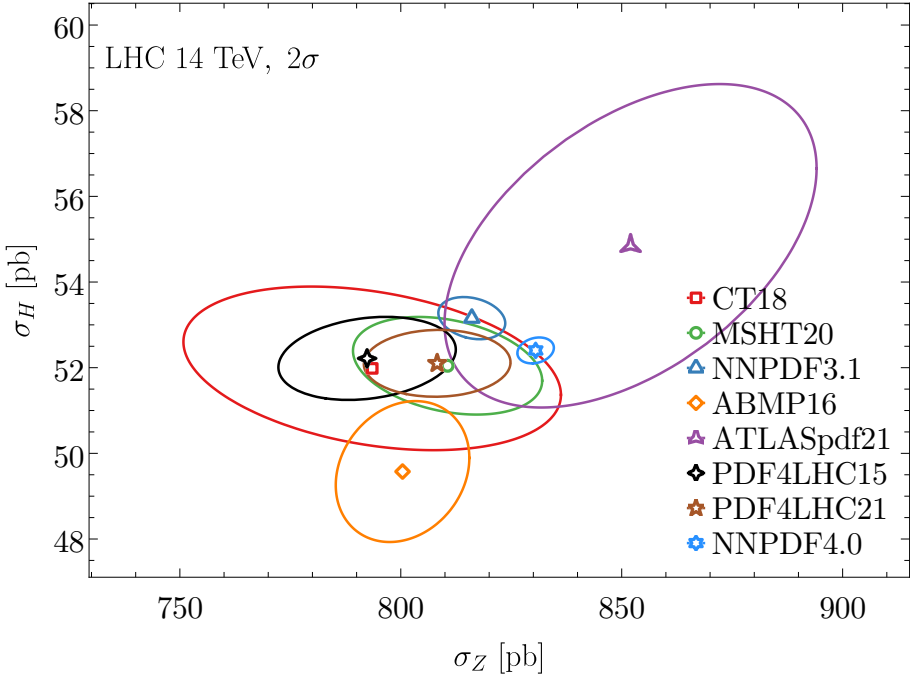
\includegraphics[width=0.45\textwidth]{ZH_xsec_wrong}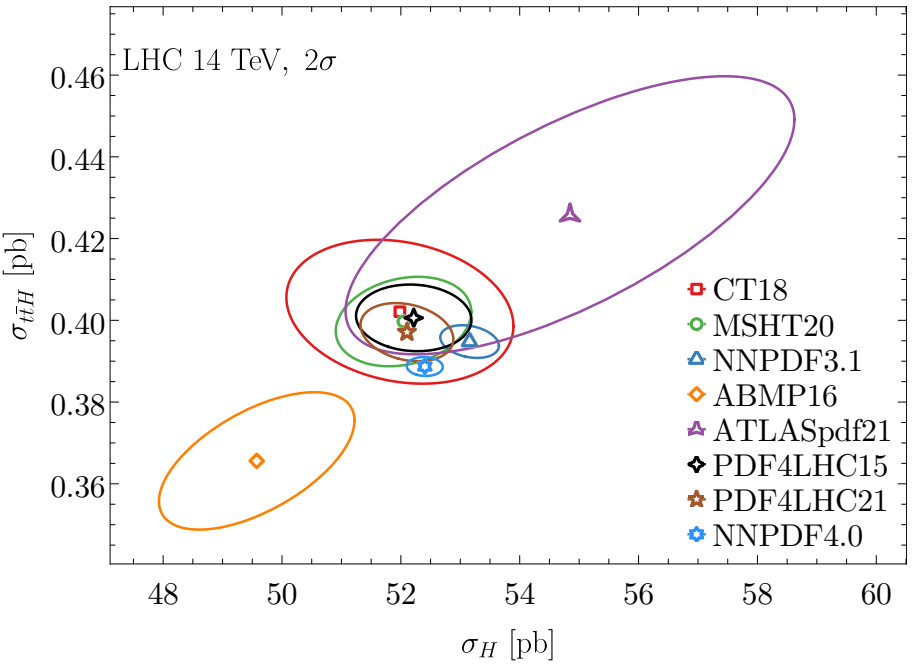
\includegraphics[width=0.45\textwidth]{HttbarH_xsec_wrong}
%                 };
%                 \begin{scope}[x={(image.south east)},y={(image.north west)}]
%                     \node[align=center, text=gray,font=\bfseries\fontsize{30}{0}\selectfont] at (0.5,0.7) {BUGGED FIGURES};
%                 \end{scope}
%         \end{tikzpicture}
%         % 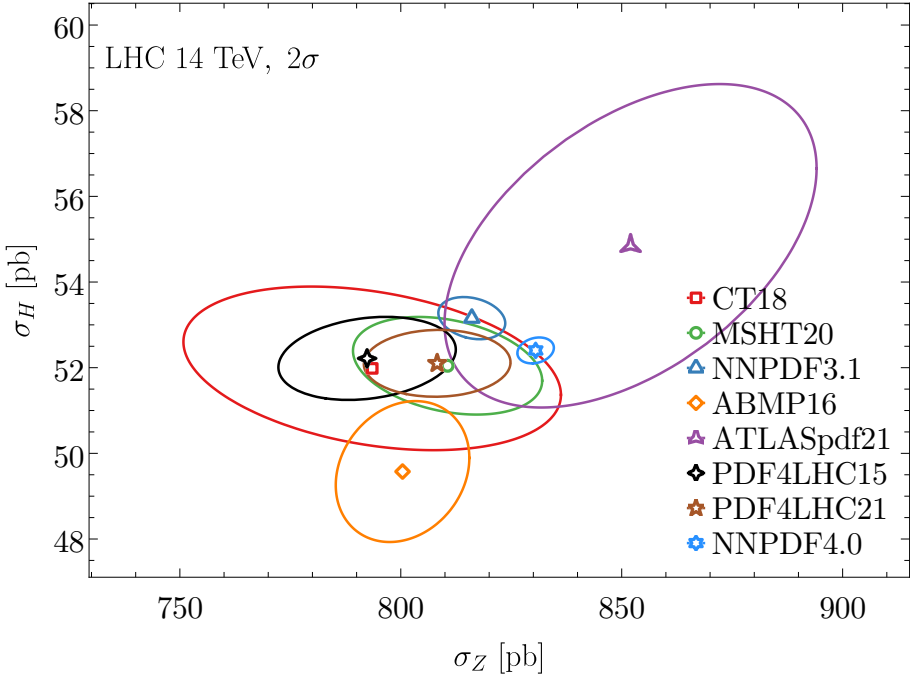
\includegraphics[width=0.45\textwidth]{ZH_xsec_wrong}
% 		% 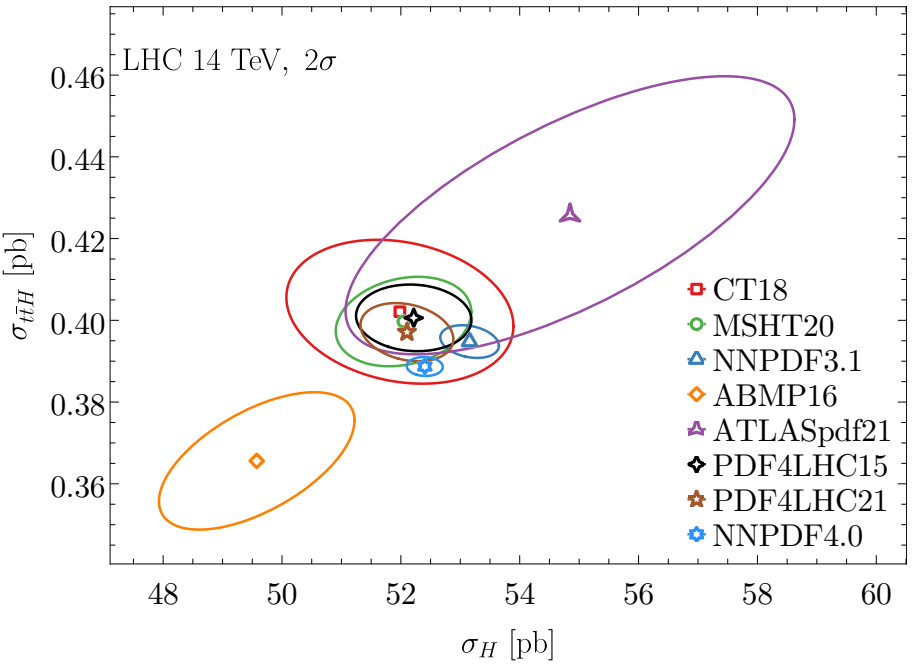
\includegraphics[width=0.45\textwidth]{HttbarH_xsec_wrong}
% 	\end{center}
%     Plots as shown in Snowmass 2021, 2203.13923\textbf{v1}\\
%     Error in the calculation of correlations for Monte Carlo PDFs!
% \end{frame}


\begin{frame}{Status of modern PDF sets}
    PDF predictions are {\bfseries consistent} but with {\bfseries different uncertainties}
	\begin{center}
		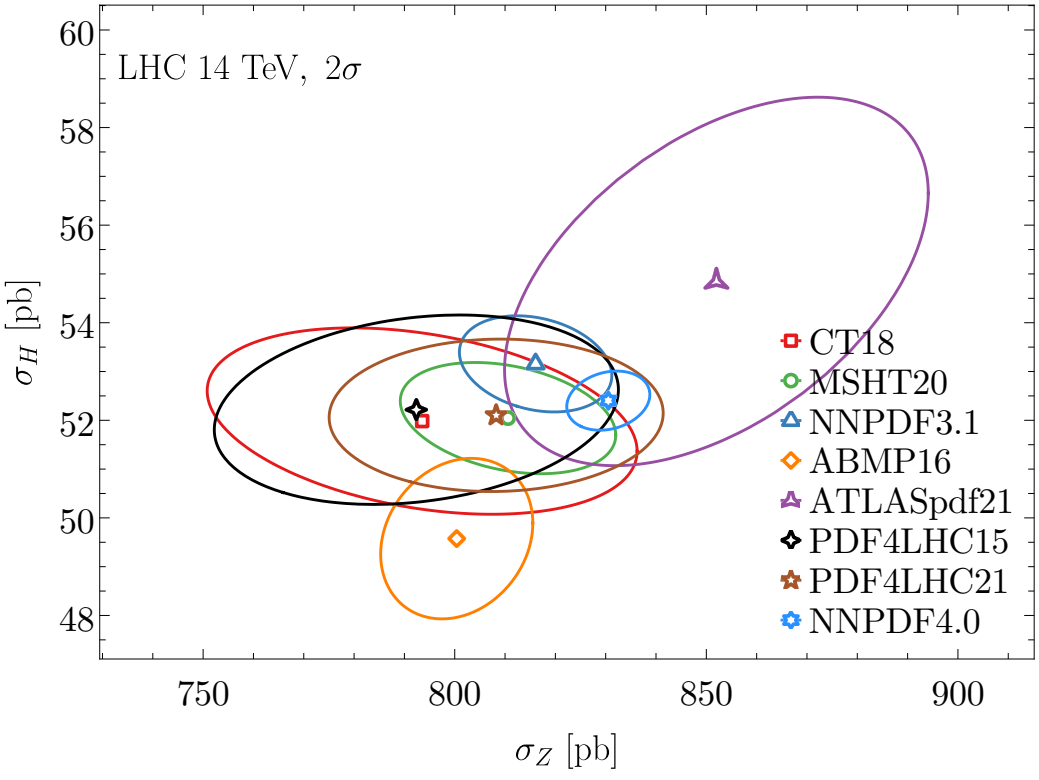
\includegraphics[width=0.45\textwidth]{ZH_xsec_fixed.png}
		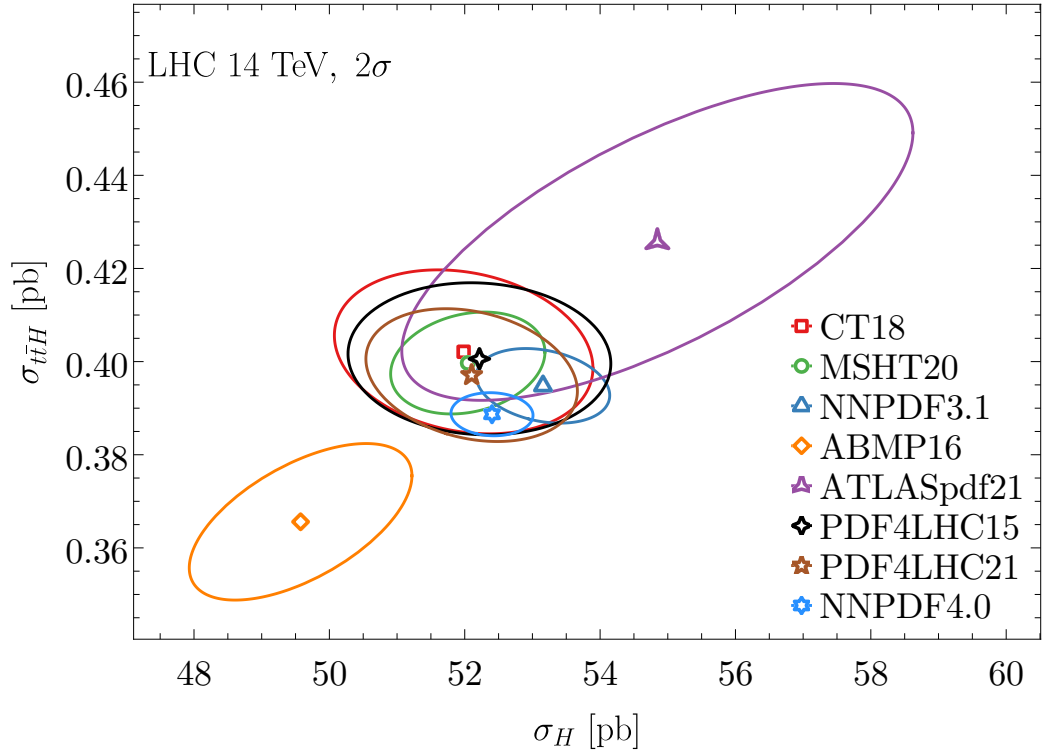
\includegraphics[width=0.45\textwidth]{HttbarH_xsec_fixed.png}
	\end{center}
    \begin{center}
	    \textbf{How is the improved precision from NNPDF3.1 to NNPDF4.0 achieved?}
	\end{center}
\end{frame}



% DATA ========================================================================
\section{Data}

% \begin{frame}{Data from NNPDF1.0 to NNPDF4.0}
% 	\begin{center}
% 		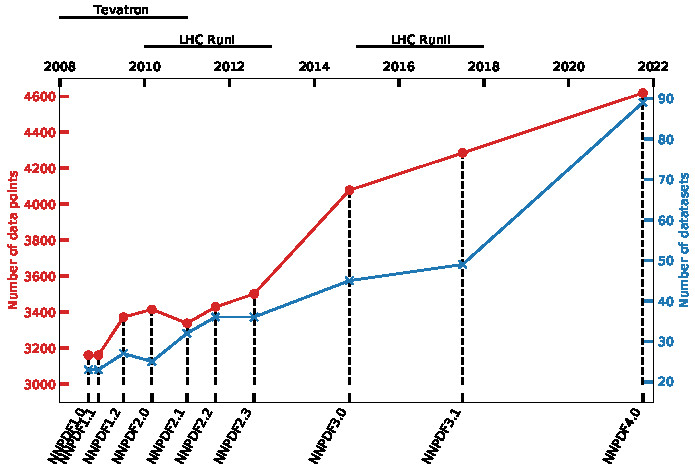
\includegraphics[width=0.5\textwidth]{NNPDF_data_history.pdf}
% 	\end{center}
% 	The number of datasets -- normally corresponding to different processes -- is generally more relevant than the number of datapoints
% \end{frame}


\begin{frame}{Experimental data in NNPDF4.0}
    \begin{columns}
        \column{0.7\linewidth}
            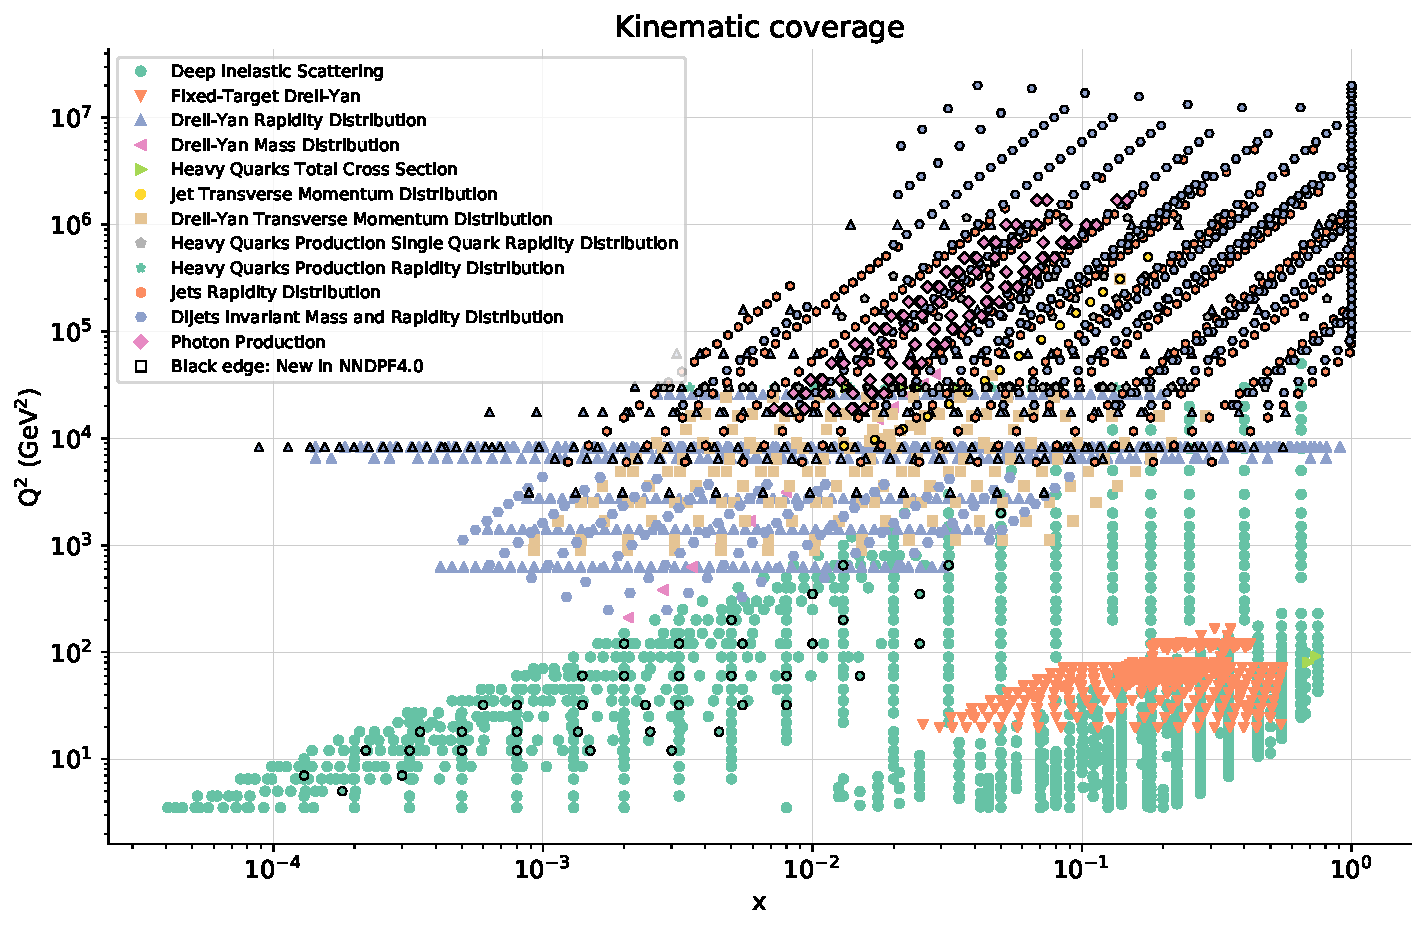
\includegraphics[width=1.0\textwidth]{Markers0_plot_xq2}
        \column{0.3\linewidth}
            More than 4000 datapoints!\\
            \vspace*{1em}
            New processes:
            \begin{itemize}
                \item direct photon
                \item single top
                \item dijets
                \item W+jet
                \item DIS jet
            \end{itemize}
    % \begin{block}{\footnotesize Theoretical improvement}
    % {\footnotesize
    % Nuclear uncertainties are included
    % }
    % \end{block}
    \end{columns}
\end{frame}



% METHODOLOGY ==================================================================
\section{Methodology}

\begin{frame}{The NNPDF4.0 model}{See  \href{https://arxiv.org/pdf/1907.05075}{\color{blue} EPJ\,C79\,(2019)\,676}}
    \begin{figure}[t]
      \centering
      \resizebox{0.8\textwidth}{!}{%
        \begin{tikzpicture}[node distance = 1.0cm]\scriptsize
        % Input node
        \node (xinput) {$\{\mathrm{xgrid}_n\}$};
    
        % PDF basis
        \coordinate [right = 1.5cm of xinput] (NNghost) {};
        \node[fitted, above = 1.0cm of NNghost, minimum width=1.7cm, minimum height=0.7cm] (pdf) { Neural Net};
        \node[fitted, below = 1.0cm of NNghost, minimum width=1.7cm, minimum height=0.7cm] (preproc) { $x^{\alpha}$ $(1-x)^{\beta}$};
        \node[above = 0.6cm of pdf, minimum width=1.7cm, minimum height=0.3cm] (fform) 
        {\color{red} {\fontsize{10pt}{0}\selectfont $\mathrm{PDF}=Ax^\alpha(1-x)^\beta \mathrm{NN}(x,\log x)$} };
    
        % PDF production
        \node[operations, fill=violet!40, minimum width=1.2cm, minimum height=0.7cm, right = 1.5cm of NNghost]
            (fitbasis) {$\overline{\mathrm{PDF}}_n$};
        \node[operations, fill=violet!40, minimum width=1.2cm, minimum height=0.7cm, right = 0.6cm of fitbasis]
            (normalizer) {normalization};
    
        % PDFs 1 to n
        \node[right = 0.9cm of normalizer] (pdfdots) {\vdots};
        \node[above = 0.7cm of pdfdots] (pdf1) {PDF$_1$};
        \node[below = 0.7cm of pdfdots] (pdfn) {PDF$_n$};
    
        % Convolutions 1 to n
        \node[right = 0.2cm of pdf1] (conv1) {$\otimes$};
        \node[right = 0.2cm of pdfn] (convn) {$\otimes$};
        \node at ($(conv1)!0.5!(convn)$) (convdots) {$\otimes$};
    
        % FK Tables 1 to n
        \node[blue, right = 0.6cm of conv1] (f1) {$\hat{\sigma}_1$};
        \node[blue, right = 0.6cm of convn] (fn) {$\hat{\sigma}_n$};
        \node[blue] at ($(f1)!0.5!(fn)$) (fd) {\vdots};
        \draw[draw=blue, rounded corners] ($(f1.north west)+(-0.1, 0.2)$) rectangle ($(fn.south east)+(0.1,-0.2)$);
            \node[above = 0.6cm of f1] (theory) {Theory};
            \coordinate [above = 0.2cm of f1] (theoryarrow) {};
    
        % Observables
        \node[right = 0.5 cm of f1] (o1) {$\mathcal{O}_{1}$};
        \node[right = 0.5 cm of fn] (on) {$\mathcal{O}_{n}$};
        \node at ($(o1)!0.5!(on)$) (od) {\vdots};
        \node[above = 0.9cm of o1] (observables) {Observables};
        \coordinate [above = 0.2cm of o1] (observablearrow) {};
    
        % Tr/Vl split
        \node[operations, right = 0.5cm of od, minimum width = 1.2cm, text width=1cm, minimum height=0.7cm]
        (trvl) {Tr/Vl split};
        \coordinate [right = 1.0cm of trvl] (ending) {};
        \path let \p1 = (ending), \p2 = (pdf)
            in node at (\x1,\y2) [n3py, minimum width = 1.2cm, minimum height=0.7cm] (tr) {$\chi^{2}_\text{tr}$};
        \path let \p1 = (ending), \p2 = (preproc)
            in node at (\x1,\y2) [n3py, minimum width = 1.2cm, minimum height=0.7cm] (vl) {$\chi^{2}_\text{vl}$};
    
        % Arrows!
        \draw[myarrow] (xinput) -- (pdf);
        \draw[myarrow] (xinput) -- (preproc);
        \draw[myarrow] (pdf) -- (fitbasis);
        \draw[myarrow] (preproc) -- (fitbasis);
        \draw[myarrow] (fitbasis) -- (normalizer);
    
        \draw[myarrow] (pdf1) -- (conv1);
        \draw[myarrow] (pdfn) -- (convn);
        \draw[myarrow] (conv1) -- ($(f1.west)-(0.2,0.0)$) ;
        \draw[myarrow] (convn) -- ($(fn.west)-(0.2,0.0)$) ;
        \draw[myarrow] ($(f1.east)+(0.2,0.0)$) -- (o1);
        \draw[myarrow] ($(fn.east)+(0.2,0.0)$) -- (on);
    
        \draw[myarrow] (trvl) -- (tr);
        \draw[myarrow] (trvl) -- (vl);
        
        \draw[myarrow] (theory) -- (theoryarrow);
        \draw[myarrow] (observables) -- (observablearrow);
        
        % Braces
        \draw[decorate, decoration={brace}, thick] (pdfn.south west) -- (pdf1.north west);
        \draw[decorate, decoration={brace},thick] (o1.north east) -- (on.south east);
        \end{tikzpicture}
      }
    \end{figure}
    % \textbf{Main changes:}
    \vspace*{2em}
    \begin{itemize}
        \item Modular \texttt{Python} codebase
        \item Freedom to use external libraries (default: \texttt{TensorFlow})
        % \item Modularity $\Rightarrow$ ability to vary all aspects of the methodology
    \end{itemize}
  \end{frame}


\begin{frame}[t]{Automated model selection}
	NNPDF aims to minimize sources of bias in the PDF:
	\begin{itemize}
	    \item Functional form $\rightarrow$ Neural Network
	    \item Model parameters $\rightarrow$ \textbf{Hyperoptimization}
	\end{itemize}
    \begin{columns}
        \begin{column}{0.48\textwidth}
            Scan over thousands of hyperparameter combinations and select the best one \\
            \vspace*{0.8em}
            {\bf k-fold cross-validation}: used to define the reward function based on a {\bf test dataset}\\ 
            \vspace*{0.8em}
            Objective function: \\
            $L=\textrm{mean}(\chi_1^2,\chi_3^2,\chi_2^2,\ldots, \chi_k^2)$
        \end{column}
        \begin{column}{0.48\textwidth}
            \begin{center}
                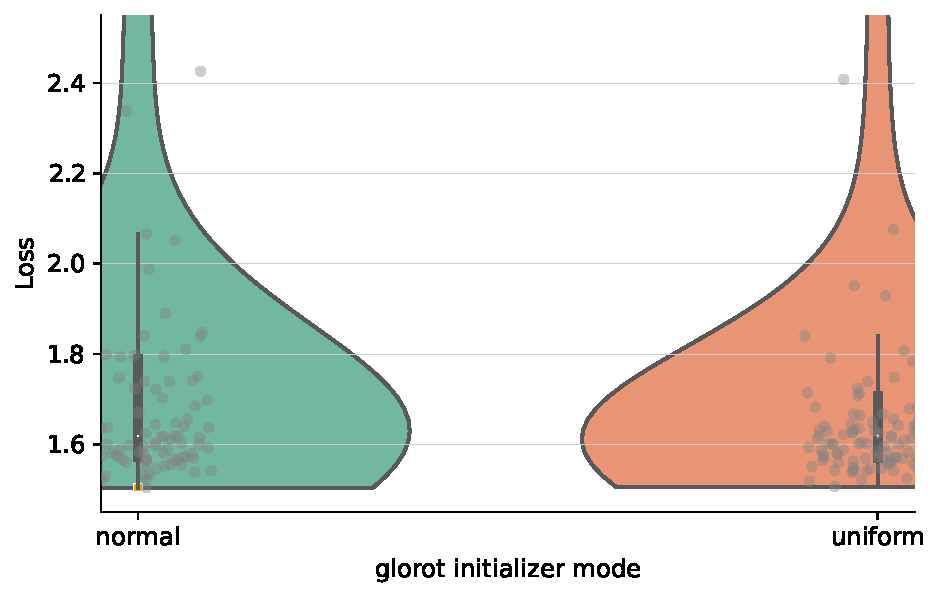
\includegraphics[width=0.48\textwidth]{sec_methodology_hyperopt_plot_initializer.pdf}
                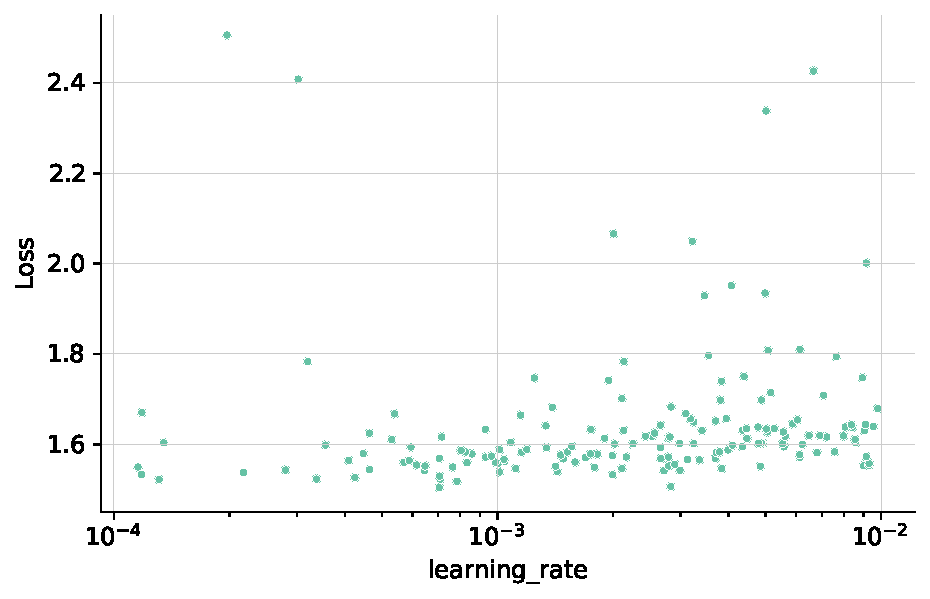
\includegraphics[width=0.48\textwidth]{sec_methodology_hyperopt_plot_lr.pdf} \\
                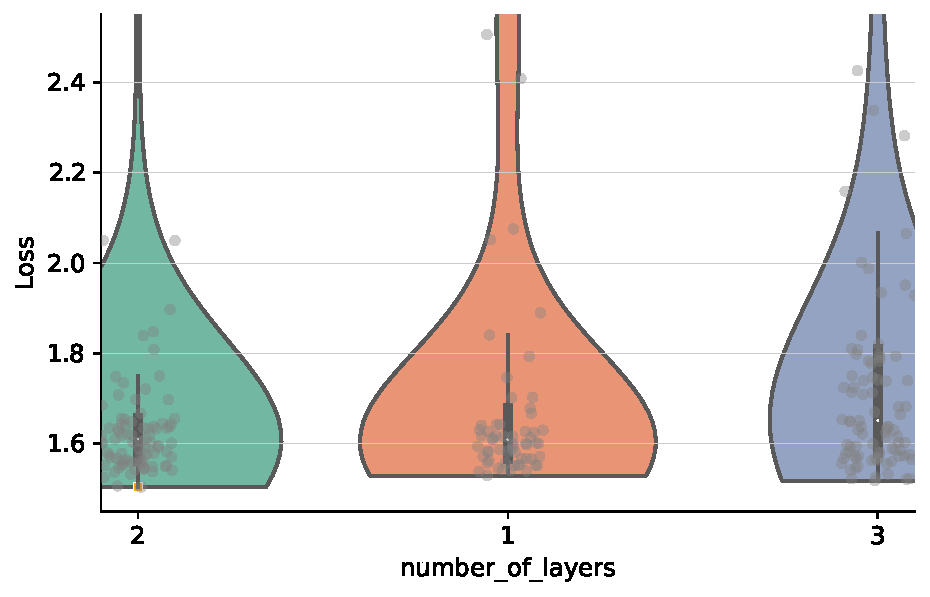
\includegraphics[width=0.48\textwidth]{sec_methodology_hyperopt_plot_number_of_layers.pdf}
                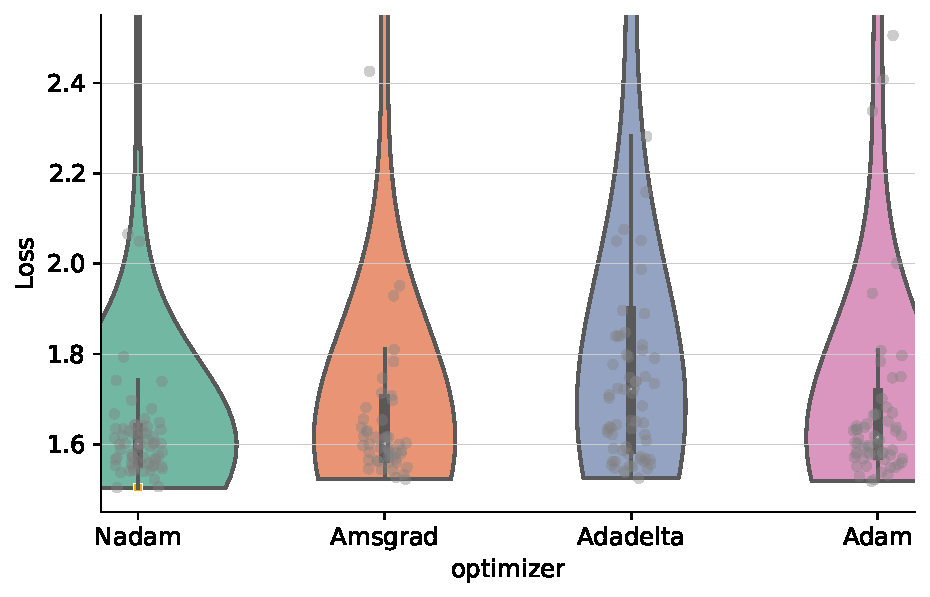
\includegraphics[width=0.48\textwidth]{sec_methodology_hyperopt_plot_optimizers.pdf}
            \end{center}
        \end{column}
    \end{columns}
\end{frame}


\begin{frame}[t]{Further methodological improvments}
    \begin{columns}[T]
        \begin{column}{0.48\textwidth}
            \begin{itemize}
                \item Improved implementation of physical constraints
                \begin{itemize}
                    \item[-] PDF \textbf{positivity}
                    \item[-] {\bfseries Integrability} of non-singlet distributions
                \end{itemize}
                % \item New fitting code
                % \begin{itemize}
                %     \item[-] Optimization based on {\bfseries Stochastic Gradient Descent} using TensorFlow
                %     \item[-] Automated selection of model {\bfseries hyperparameters}
                %     % \item[-] Modular python code
                % \end{itemize}
                \item Extended validation of PDFs
                \begin{itemize}
                    \item[-] Explicit check of {\bfseries basis independence}
                    \item[-] {\bfseries Test uncertainties} using closure and future test
                \end{itemize}
            \end{itemize}
        \end{column}
        \begin{column}{0.48\textwidth}
            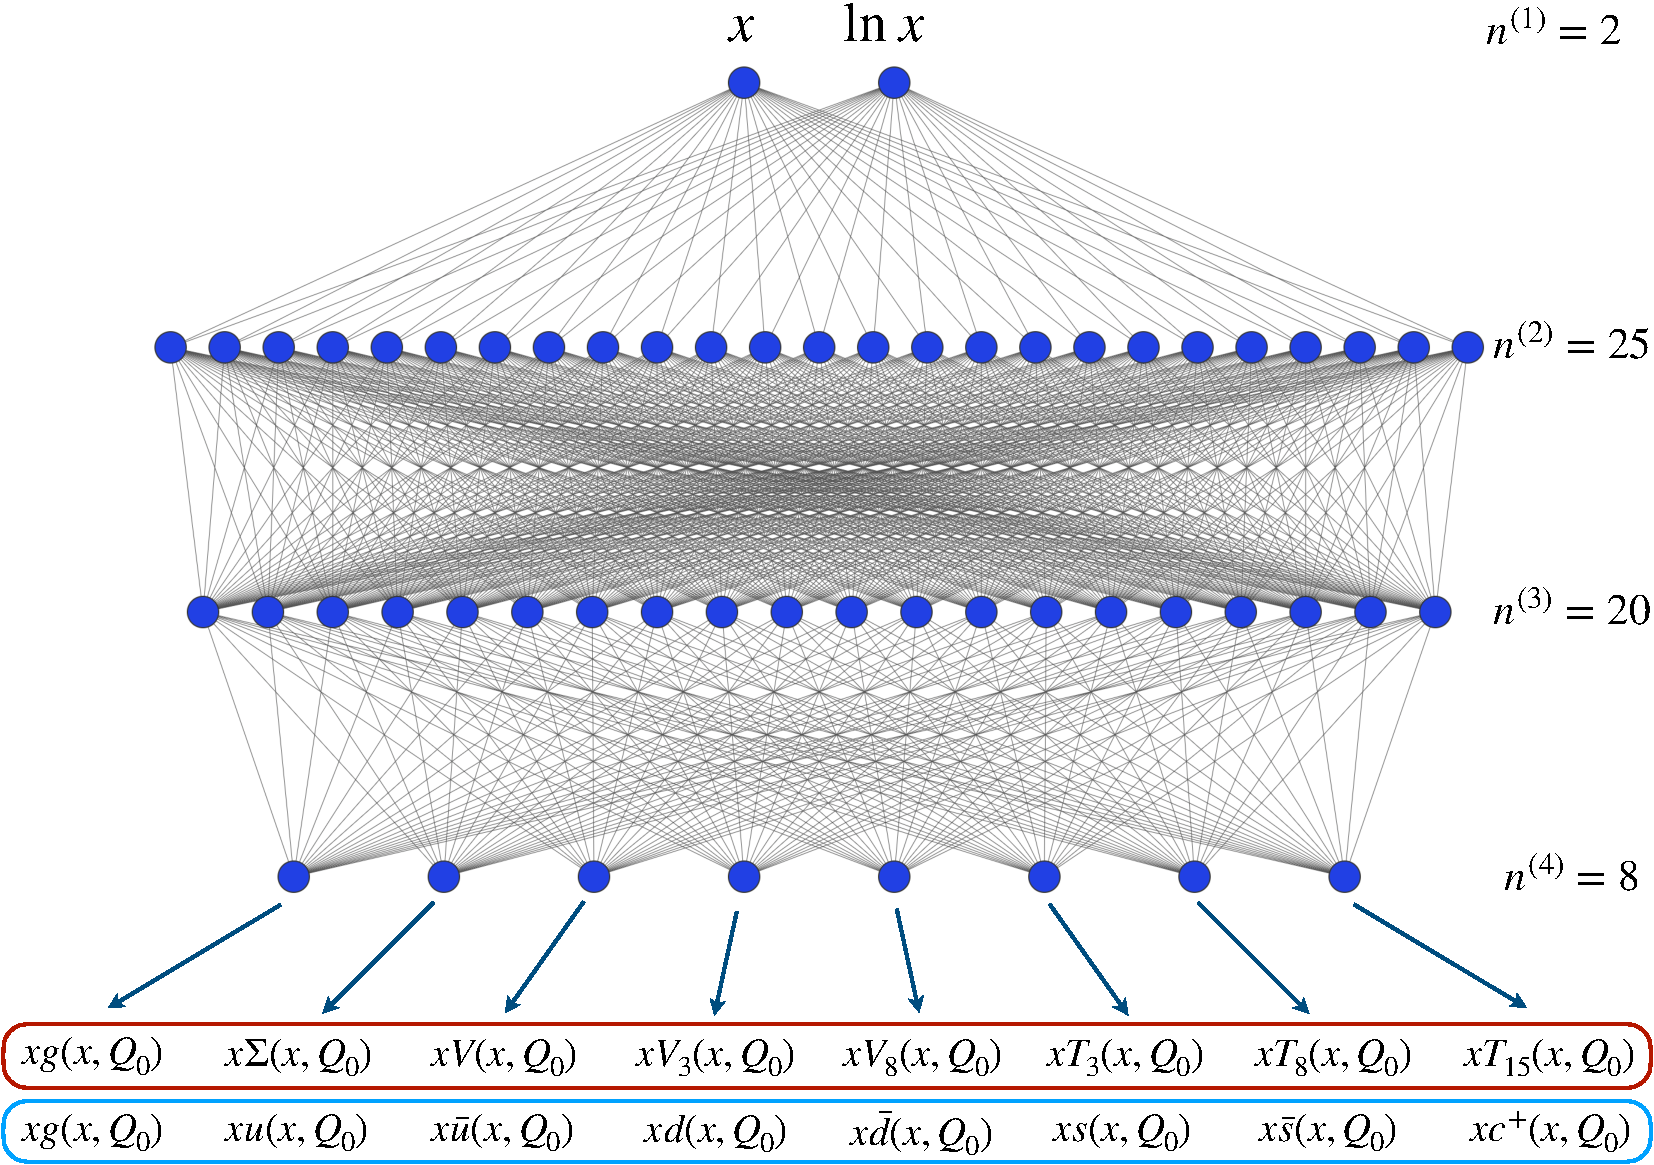
\includegraphics[width=1.0\textwidth]{NNarch}
            \begin{equation*}
                f_{i}\left(x, Q_{0}\right)=x^{-\alpha_{i}}(1-x)^{\beta_{i}} \mathrm{NN}_{i}(x)
            \end{equation*}
        \end{column}
    \end{columns}
\end{frame}



% VALIDATION ===================================================================
\section{Validation}


\begin{frame}[t]{Future tests}{See \href{https://arxiv.org/pdf/2111.05787.pdf}{\color{blue}Acta Phys.Polon.B 52 (2021) arxiv:2103.08606}}

    \begin{columns}
        \column{0.60\linewidth}
        \begin{enumerate}
            \item Take a historic dataset \\ e.g. pre-HERA or pre-LHC
            \item Perform fit
            \item Compare predictions to ``future'' data
        \end{enumerate}
        \centering
        % 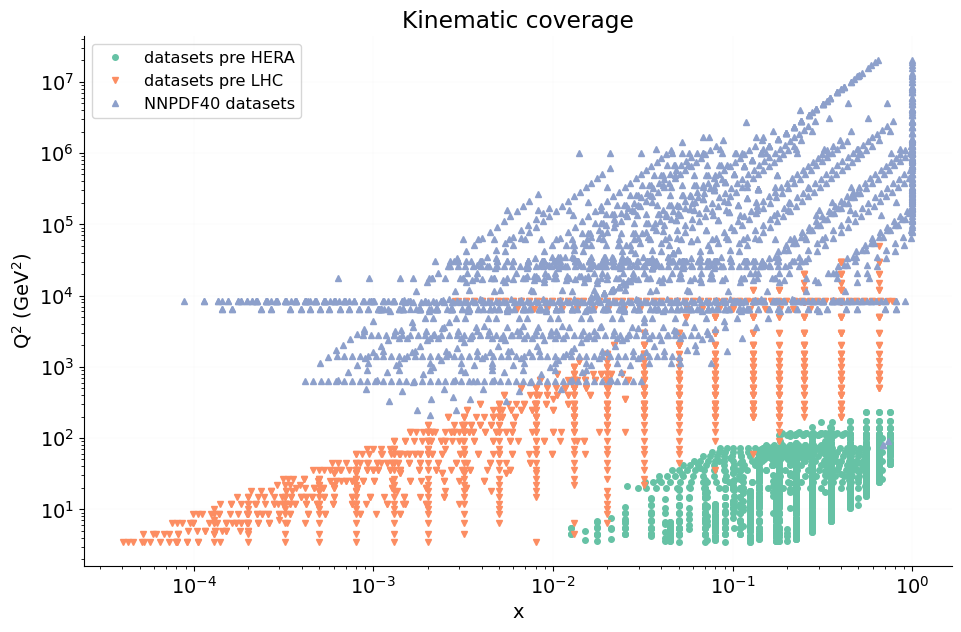
\includegraphics[width=0.7\textwidth]{kincov}
        \column{0.46\linewidth}
        \vspace{-1cm}
        \only<1>{
            \begin{table}
                \tiny
                \centering
                \caption*{\scriptsize $\chi^{2}/N$ (only exp. covmat)}
                \begin{tabular}{c | c c c} \toprule
                    (dataset) & NNPDF4.0 & pre-LHC & pre-Hera  \\ \midrule
                    pre-HERA  & 1.09 & 1.01 & 0.90 \\
                    pre-LHC   & 1.21 & 1.20 & \hlme{23.1} \\
                    NNPDF4.0  & 1.29 & \hlme{3.30} & \hlme{23.1} \\
                    \bottomrule
                \end{tabular}
            \end{table}
        }
        \only<2>{
            \begin{table}
                \tiny
                \centering
                \caption*{\scriptsize $\chi^{2}/N$ (exp. and PDF covmat)}
                \begin{tabular}{c | c c c} \toprule
                    (dataset) & NNPDF4.0 & pre-LHC & pre-Hera  \\ \midrule
                    pre-HERA  &  & & 0.86 \\
                    pre-LHC   &  & 1.17 & \hlme{1.22} \\
                    NNPDF4.0  & 1.12 & \hlme{1.30} & \hlme{1.38} \\
                    \bottomrule
                \end{tabular}
            \end{table}
        }


        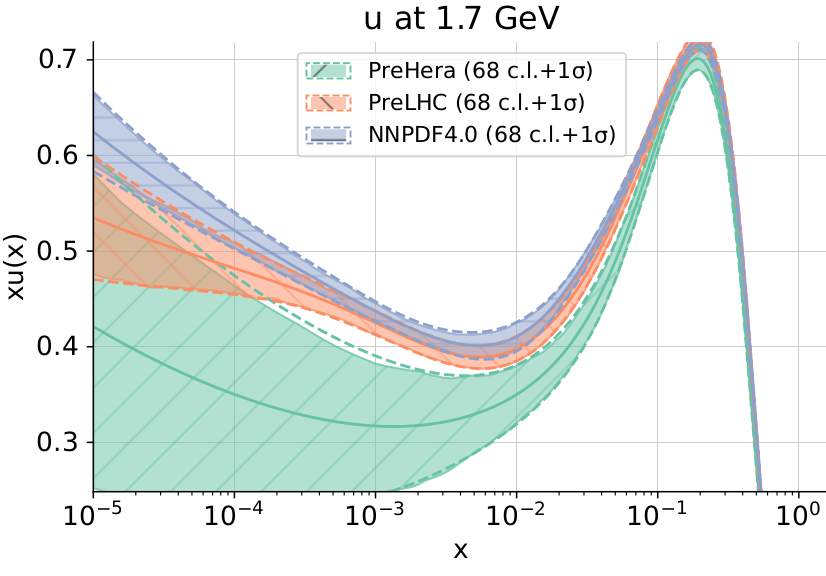
\includegraphics[width=0.9\textwidth]{diffu}
    \end{columns}
        \only<2>{\small The total uncertainty increases, and accommodates for difference between predictions and new data.}
\end{frame}


\begin{frame}[t]{Sampling for solutions}
    Is the sampling of the PDF uncertainty of an experimental observable truly representative of all acceptable solutions?\\
    \begin{columns}
        \begin{column}{0.4\textwidth}
            \begin{figure}
                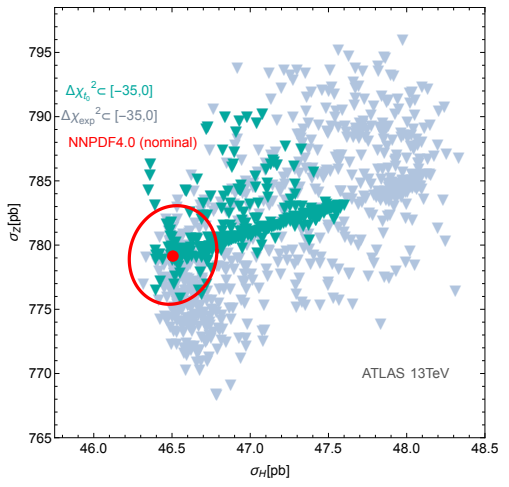
\includegraphics[width=0.9\textwidth]{cteq}
                \caption*{arXiv:2205.10444, A. Courtoy et. al.}
            \end{figure}
        \end{column}
        \begin{column}{0.6\textwidth}
            \begin{itemize}
                \item A "hopscotch scan" to search for solutions with equal or better $\chi^2$
                \item All solutions fall within the NNPDF4.0 distribution
            \end{itemize}
            \begin{figure}
                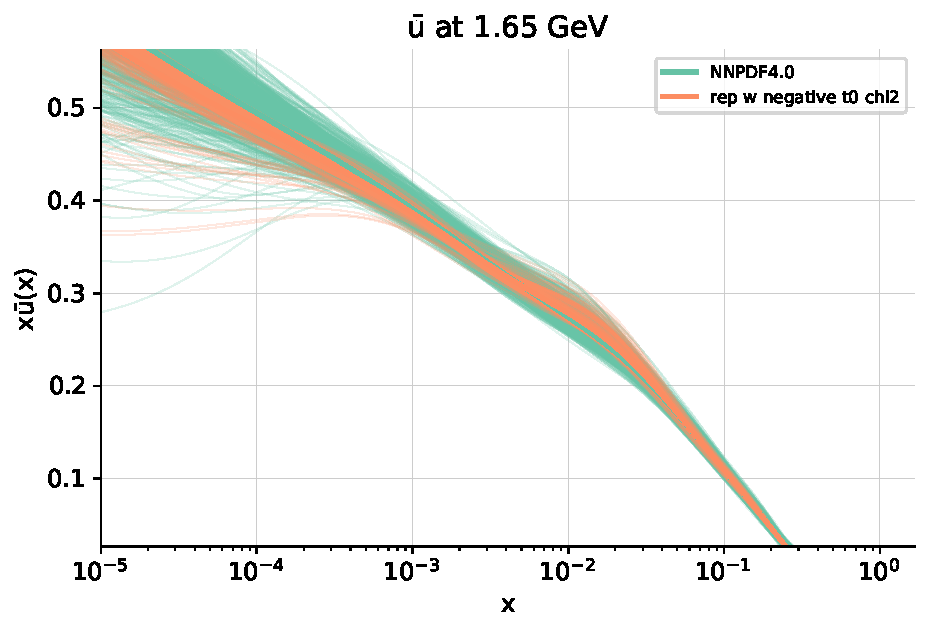
\includegraphics[width=0.75\textwidth]{cteq_ubar}
            \end{figure}
        \end{column}
    \end{columns}
\end{frame}



% PHENO ========================================================================
\section{Phenomenology}

\begin{frame}[t]{LHC phenomenology}
    \begin{center}
        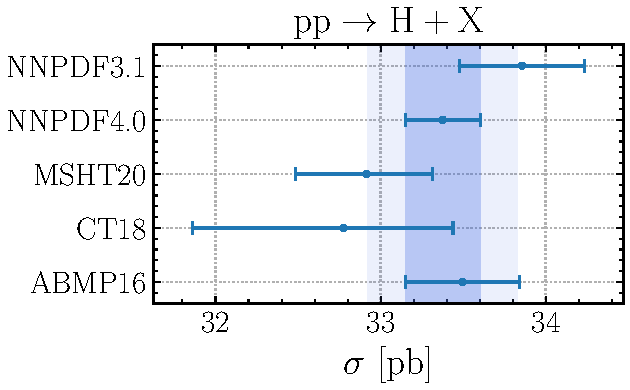
\includegraphics[width=0.48\textwidth]{NNPDF_H_14TEV_40_PHENO-integrated}
        \hspace*{0.02\textwidth}
        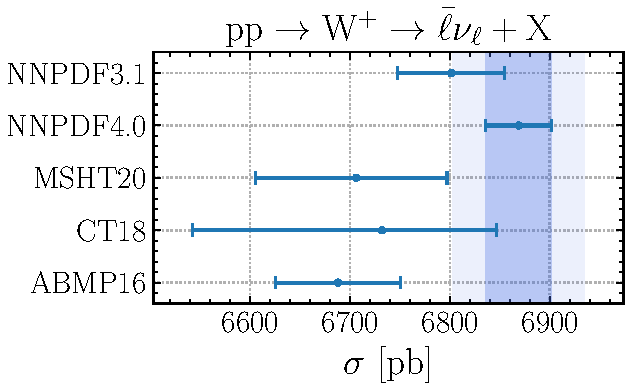
\includegraphics[width=0.48\textwidth]{NNPDF_WP_14TEV_40_PHENO-integrated}\\
        \vspace*{1em}
        \begin{itemize}
            \item Agreement between NNPDF4.0, CT18, and MSHT20 at two-sigma level
            \item NNPDF4.0 is the most precise in the data region
        \end{itemize}
    \end{center}
\end{frame}


\begin{frame}{DY at high energies [R.D Ball et. al., in preparation]}
    \vspace*{-3em}
    \begin{columns}
        \begin{column}{0.66\textwidth}
            \begin{column}{0.5\textwidth}
                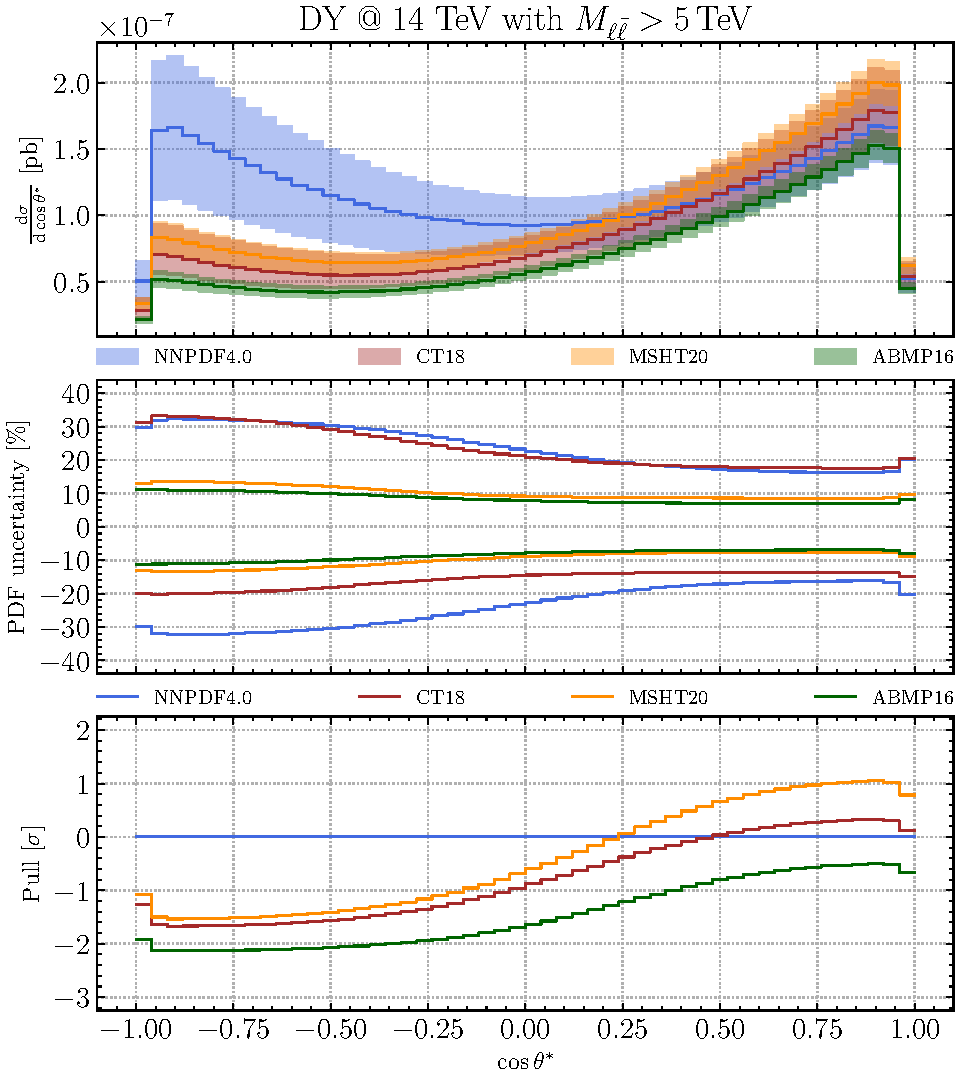
\includegraphics[width=\textwidth]{CMS_DY_14TEV_MLL_5000_COSTH}
            \end{column}
            \begin{column}{0.5\textwidth}
                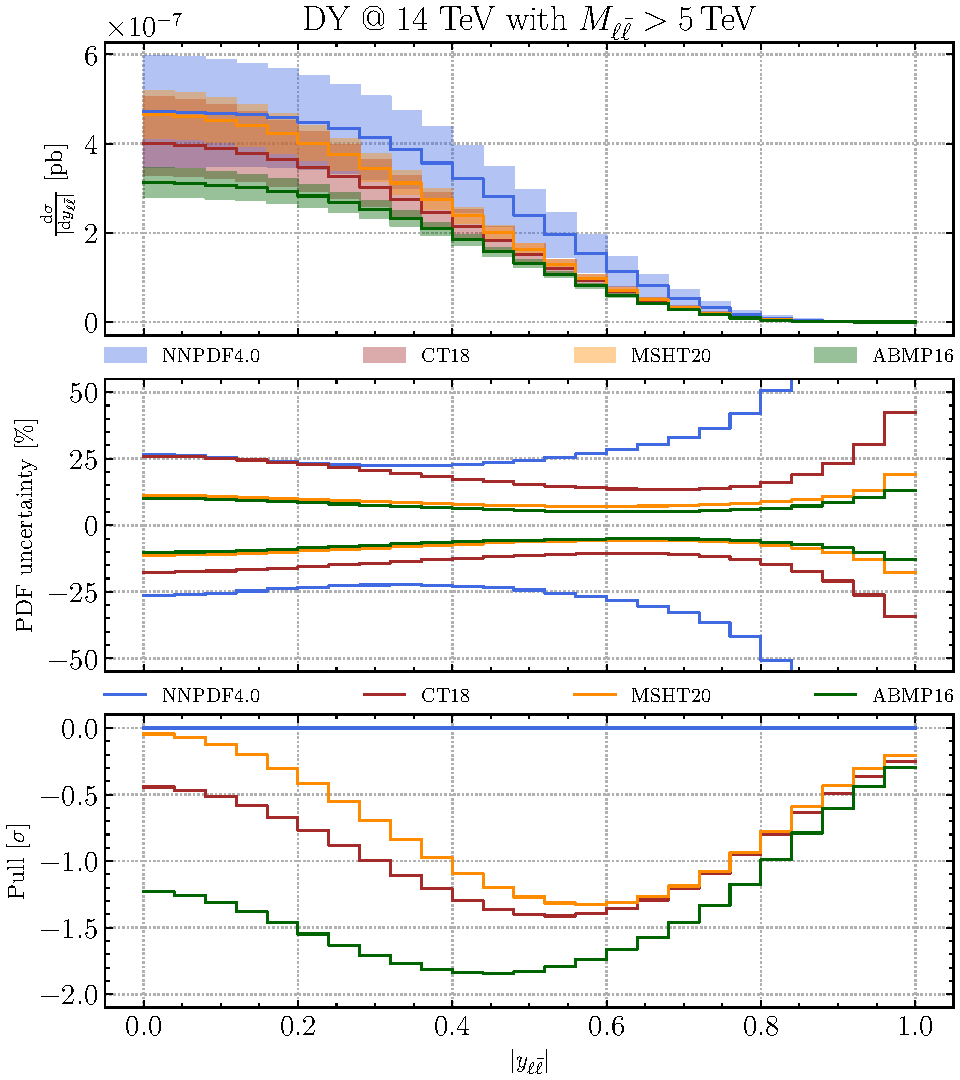
\includegraphics[width=\textwidth]{CMS_DY_14TEV_MLL_5000_YLL}
            \end{column}
        Large uncertainties for poorly known large-$x$ PDFs due to \textbf{flexibility} of the neural network
        \end{column}
        \begin{column}{0.33\textwidth}
            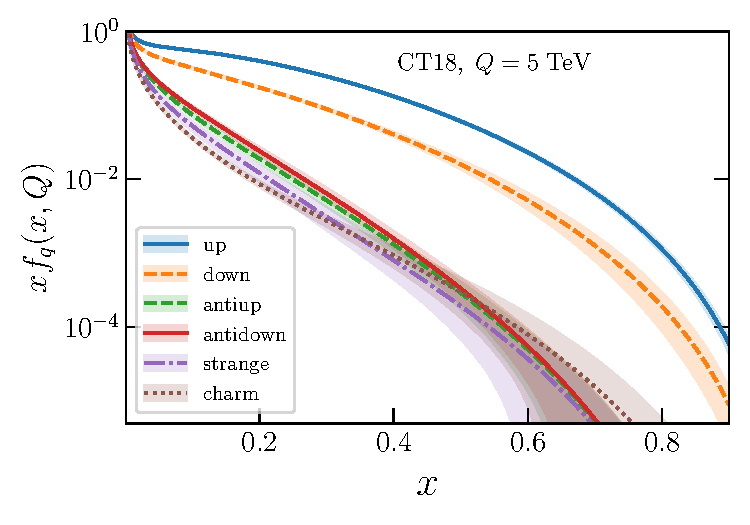
\includegraphics[width=0.75\textwidth]{pdfplot-abslargex-ct18}\\
            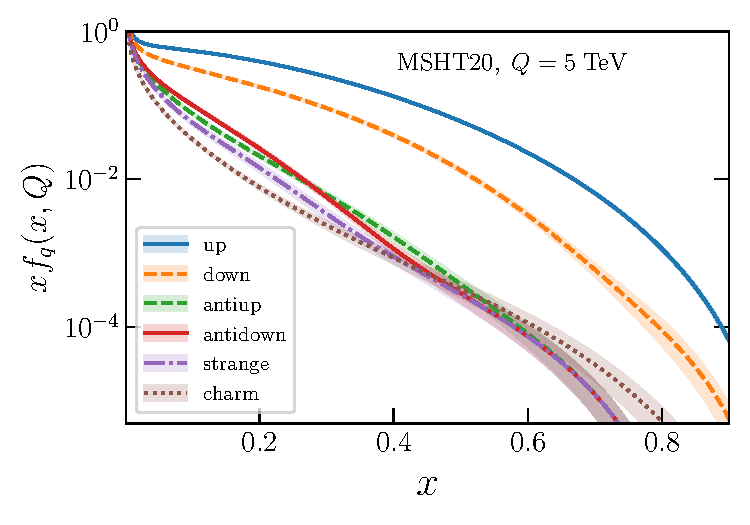
\includegraphics[width=0.75\textwidth]{pdfplot-abslargex-msht20}\\
            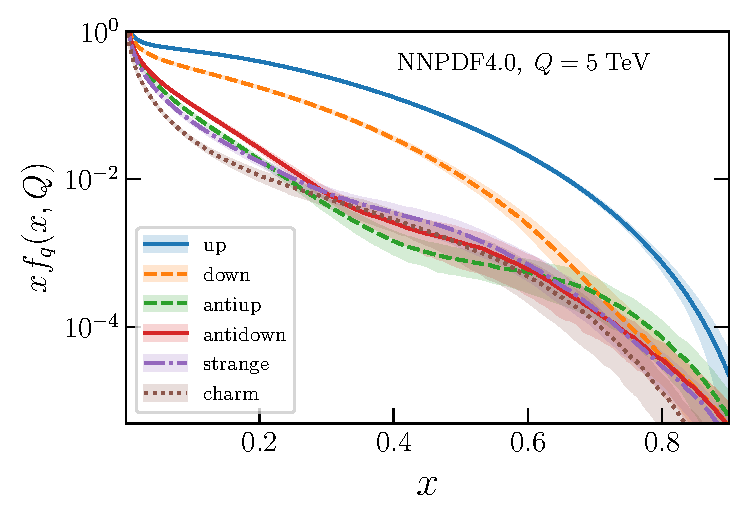
\includegraphics[width=0.75\textwidth]{pdfplot-abslargex-nnpdf40}
        \end{column}
    \end{columns}
    \centering

\end{frame}



% DELIVERY ====================================================================
% \section{Open-source code}
% \begin{frame}[t]{The open-source NNPDF code}
%     The full NNPDF code has been made public along with user friendly documentation\\
%     \vspace*{1em}
%     This includes: fitting, hyperoptimization, theory, data processing, visualization\\
%     \vspace*{1em}
%     It is possible to reproduce all results of NNPDF4.0 and more!\\
%     \vspace*{2em}
%     \begin{block}{}
%         \centering
% 		\href{https://link.springer.com/article/10.1140/epjc/s10052-021-09747-9}{Eur.Phys.J.C 81 (2021) 10, 958} \\
% 		\url{https://github.com/NNPDF/nnpdf} \\
% 		\url{https://docs.nnpdf.science}
%     \end{block}
% \end{frame}




% CONCLUSION ===================================================================
\section{Summary}
\begin{frame}[t]{Summary}
    \begin{itemize}
        \item NNPDF4.0 is the latest release in the NNPDF family of PDF sets
        \item 44 {\bfseries new datasets} from many new processes are included
        \item {\bfseries Improved methodology} with Stochastic Gradient Descent and hyperoptimization
        \item {\bfseries Validation} of PDF uncertainties using closure test, future test and parametrization basis independence
        \item[$\Rightarrow$] NNPDF4.0 achieves a high precision in the data region while simultaneously being flexible in the large-$x$ region
    \end{itemize}
	\vspace*{1em}
    \begin{block}{}
        \centering
        \textbf{The NNPDF code has been made publicly available!}\\
		\href{https://link.springer.com/article/10.1140/epjc/s10052-021-09747-9}{Eur.Phys.J.C 81 (2021) 10, 958} \\
		\url{https://github.com/NNPDF/nnpdf} \\
		\url{https://docs.nnpdf.science}
    \end{block}

    \vspace*{1em}
    \only<2>{
    \begin{center}
        {\Large \textbf{Thank you!}}
    \end{center}
    }
\end{frame}



\begin{frame}{Determination of the photon PDF}
  \begin{columns}[T]
    \begin{column}{0.59\textwidth}
      Initially the photon PDF has been determined in different ways:
      \begin{itemize}
        \item physical model: sensitive to underlying model
        \item fitting: data does not provide strong constraints
      \end{itemize}

      \vspace*{0.5em}
      However with the LUXqed approach it can be computed perturbatively \\
      based on the observation that the heavy-lepton production cross-section can be written in two ways:
      \begin{itemize}
        \item in terms of structure functions $F_2$, $F_L$
        \item in terms of PDFs (including the photon)
      \end{itemize}

      \vspace*{0.5em}
      luxQED result {\color{gray}\small[Manohar, Nason, Salam, Zanderighi: 1607.04266, 1708.01256]}:
      \vspace*{-0.8em}
      \begin{equation*}
        \begin{split}
          & x \gamma(x, \mu^2)
          =
          \frac{2}{\alpha (\mu^2)} \int\limits_x^1 \frac{dz}{z}
          \Biggl\{ \int_{m_p^2x^2 \over 1-z}^{\mu^2 \over 1-z} \frac{dQ^2}{Q^2}
          \alpha^2(Q^2) \Biggl[ -z^2 F_L(x/z, Q^2) \\
          & + \left( z P_{\gamma q}(z) + \frac{2 x^2 m_p^2}{Q^2} \right)
          F_2(x/z, Q^2)\Biggr] - \alpha^2(\mu^2) z^2 F_2(x/z, \mu^2)\Biggr\}
        \end{split}
      \end{equation*}
    \end{column}

    \begin{column}{0.39\textwidth}
      \vspace*{-2.5em}
      \begin{figure}
        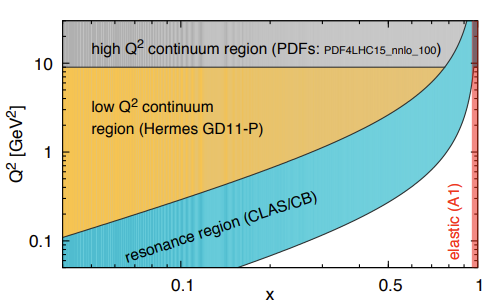
\includegraphics[width=0.89\textwidth]{figures/dataluxqed.png}
        \caption*{Input to construct $F_2$ and $F_L$}
        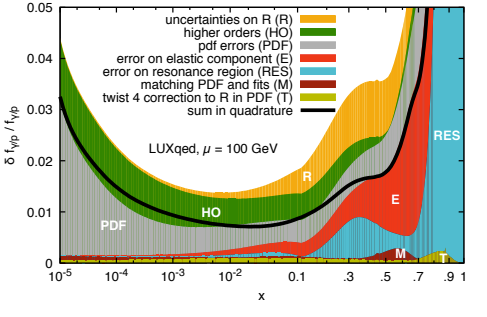
\includegraphics[width=0.89\textwidth]{figures/luxQED_uncs.png}
        \caption*{Sources of uncertainty}
      \end{figure}
    \end{column}
  \end{columns}
\end{frame}


\begin{frame}{LUXqed PDF determinations}
  LUXqed has been used in all of the most recent QED PDFs:
  \begin{itemize}
      \item LUXqed\_plus\_PDF4LHC15 {\color{gray}\small [1607.04266]}
      \item LUXqed17\_plus\_PDF4LHC15 {\color{gray}\small [1708.01256]}
      \item MMHT2015qed {\color{gray}\small [1907.02750]}
      \item NNPDF3.1luxQED {\color{gray}\small [1712.07053]}
      \item CT18lux and CT18qed {\color{gray}\small [2106.10299]}
      \item MSHT20QED {\color{gray}\small [2111.05357]}
      \item MSHT20qed\_an3lo {\color{gray}\small [2312.07665]}
      \item NNPDF4.0QED {\color{gray}\small [2401.08749 ]}
  \end{itemize}
\end{frame}

% \begin{frame}{Results: photon PDF and luminosity}
%   \begin{center}
%     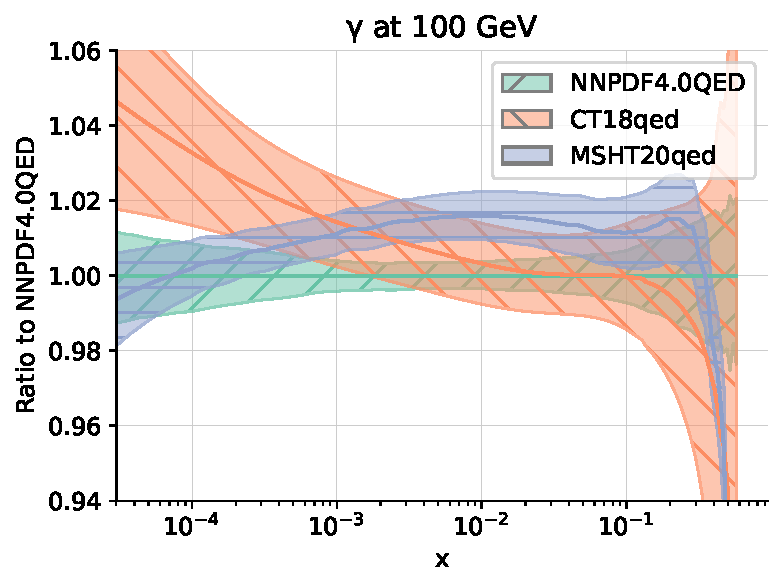
\includegraphics[width=0.3\textwidth]{figures/photon_comparison.pdf}
%     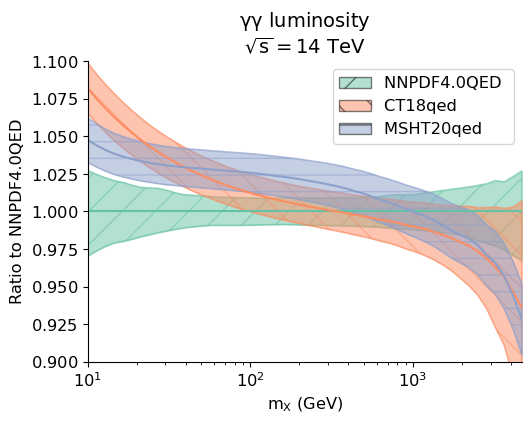
\includegraphics[width=0.3\textwidth]{figures/pp_lumi_comparison.png}
%     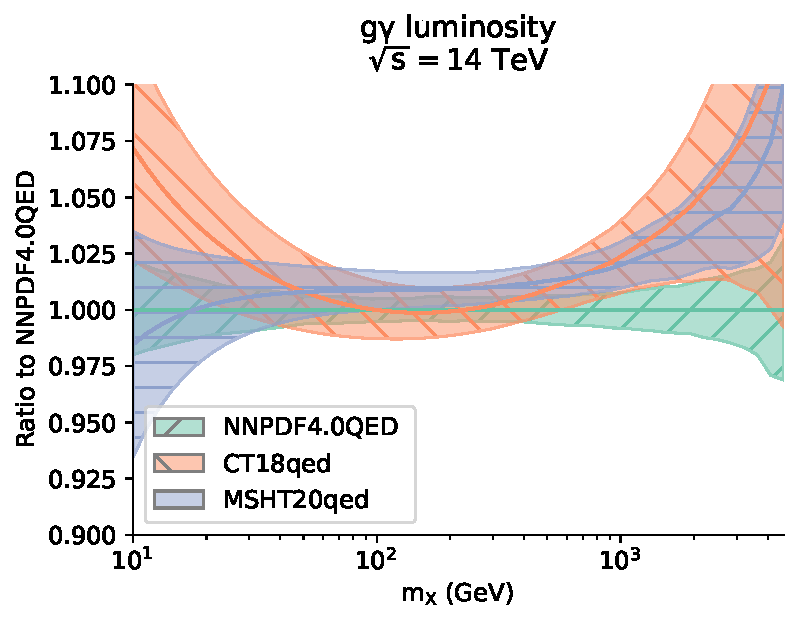
\includegraphics[width=0.3\textwidth]{figures/gp_lumi_comparison.pdf}
%   \end{center}
%   \begin{itemize}
%     \item Because all groups use the luxQED formalism, the photon PDFs agree at percent level
%     \item Luminosity generally in agreement, but differ at very small and very large invariant mass
%   \end{itemize}
% \end{frame}


% ============================================================================


\begin{frame}{Incomplete higher order uncertainties covmat}
  \begin{itemize}
    \item We construct an IHOU matrix following a similar approach by varying the subleading functions
    \item IHOU are independent of MHOU so the uncertainties are added in quadrature
    $$C = C_\mathrm{exp}+C_\mathrm{MHOU}+C_\mathrm{IHOU}$$
  \end{itemize}

  \begin{columns}
    \begin{column}{0.49\textwidth}
      \begin{figure}[!t]
        \centering
        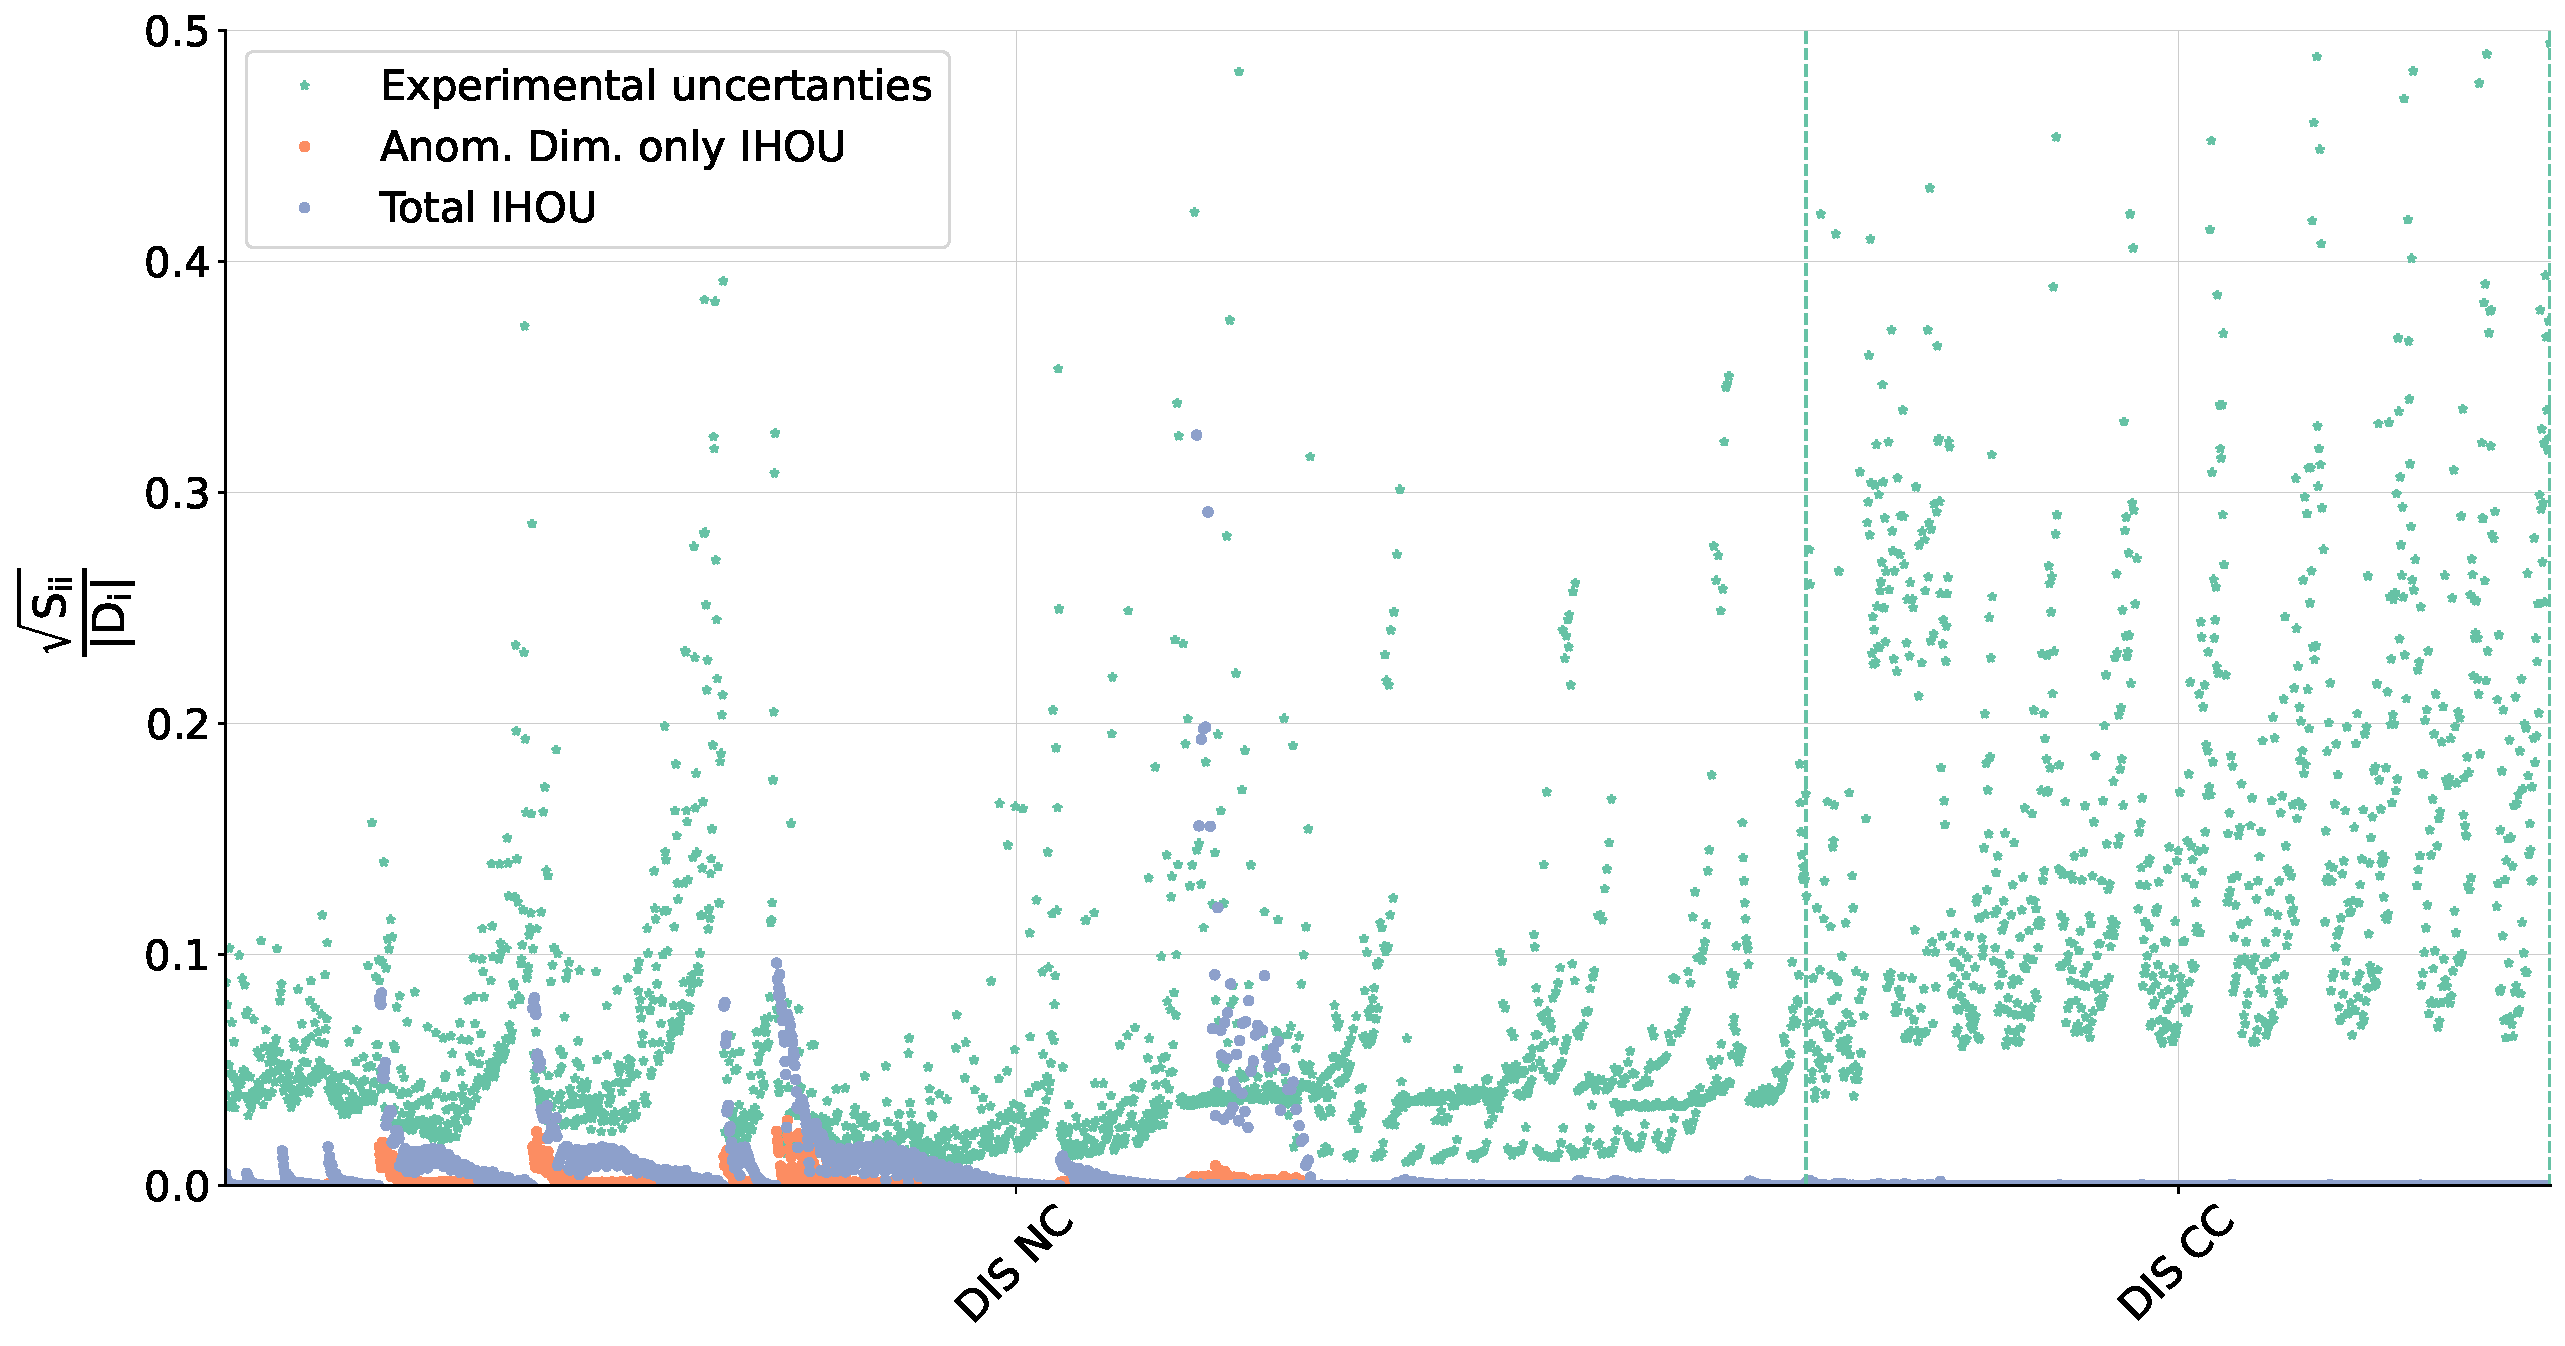
\includegraphics[width=.9\textwidth]{figures/diag_cov_dis_ihou.pdf}
        \caption*{IHOU have a large effect on small-$x$, low-$Q$ DIS data
        }
      \end{figure}
    \end{column}
    \begin{column}{0.49\textwidth}
      \begin{figure}[!t]
        \centering
        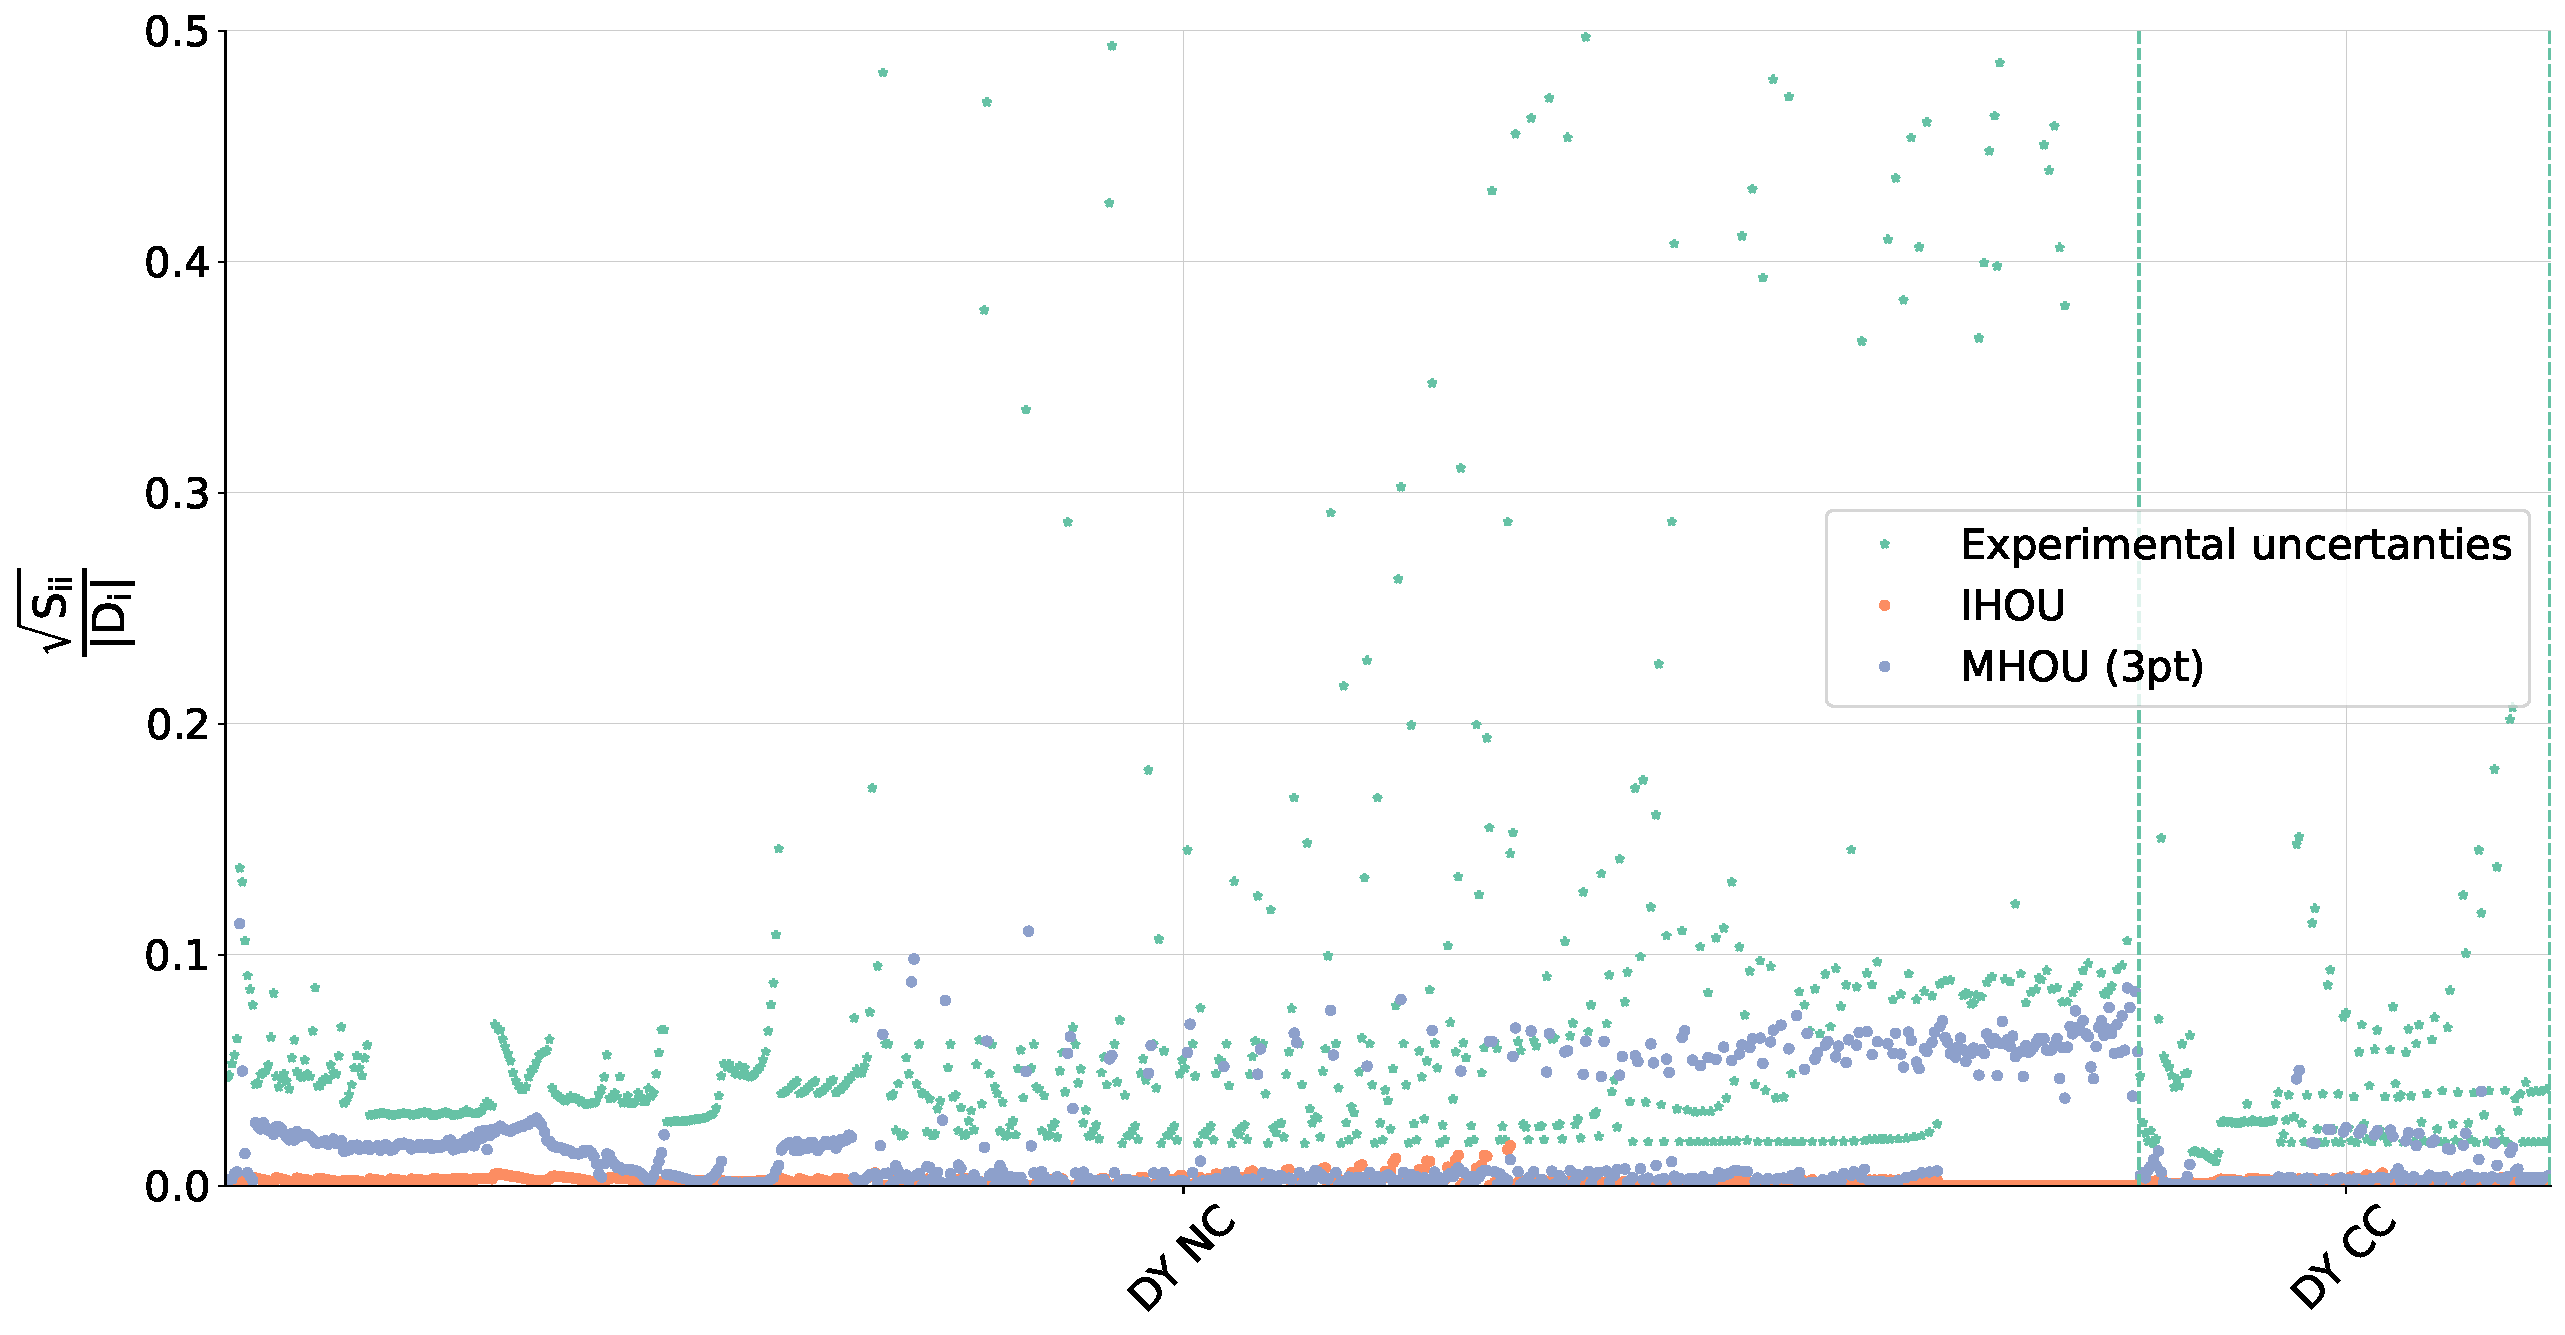
\includegraphics[width=.9\textwidth]{figures/diag_cov_dy_ihou_3pt_mhou.pdf}
        \caption*{NNLO MHOU included where N3LO not available \\
          MHOU can similar magnitude as the experimental uncertainty
        }
      \end{figure}
    \end{column}
  \end{columns}


\end{frame}

% \begin{frame}{Magnitude of theory uncertainties}
% % show that for certain processes th unc is of same size as exp unc.
% \end{frame}

% ============================================================================

\begin{frame}{Impact of MHOUs at N3LO}
  \begin{figure}[!t]
    \centering
    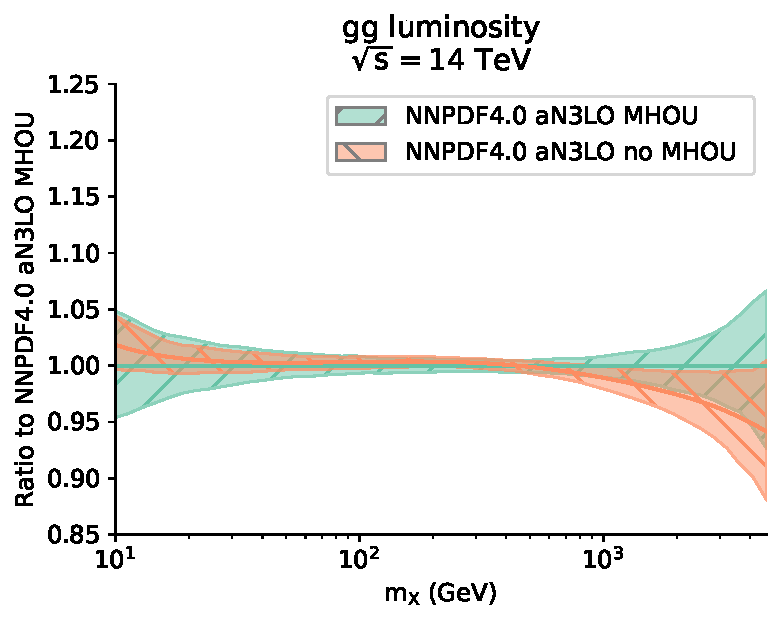
\includegraphics[width=0.45\textwidth]{figures/gg_plot_lumi1d.pdf}
    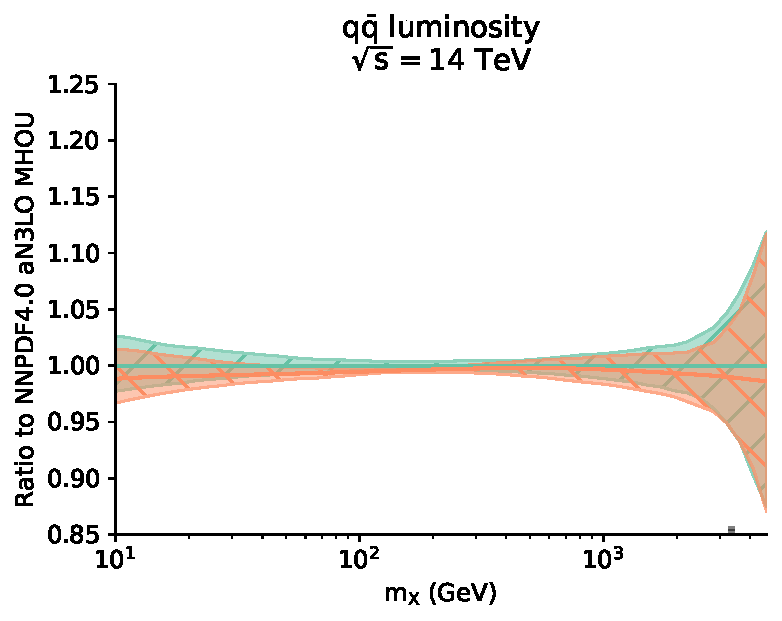
\includegraphics[width=0.45\textwidth]{figures/qqbar_plot_lumi1d.pdf}
  \end{figure}
  \begin{itemize}
    \item Non-negligible impact of MHOUs even at N3LO
    \item[$\Rightarrow$] reason to include exact N3LO calculations for hadronic processes
  \end{itemize}
\end{frame}


% \begin{frame}{Comparison to MSHT20}
%   \begin{figure}[!t]
%     \centering
%     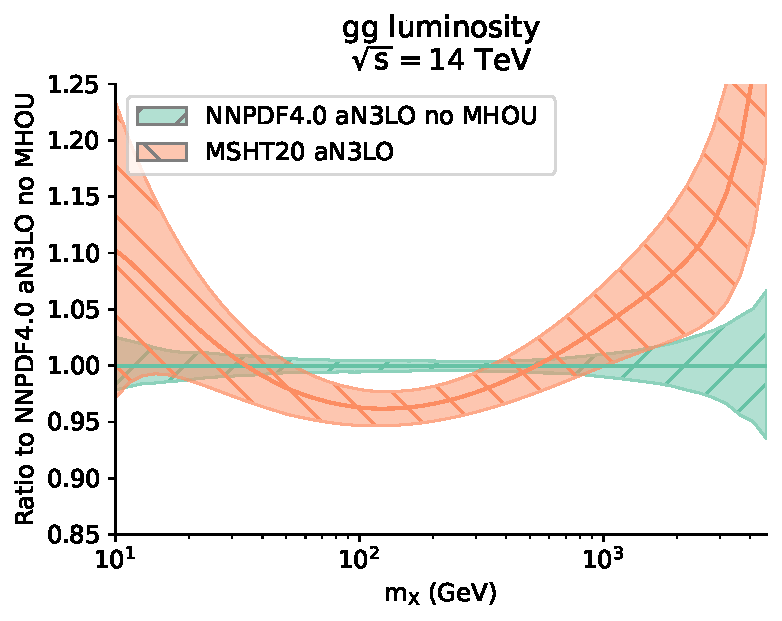
\includegraphics[width=0.45\textwidth]{figures/gg_plot_lumi1d_msht20.pdf}
%     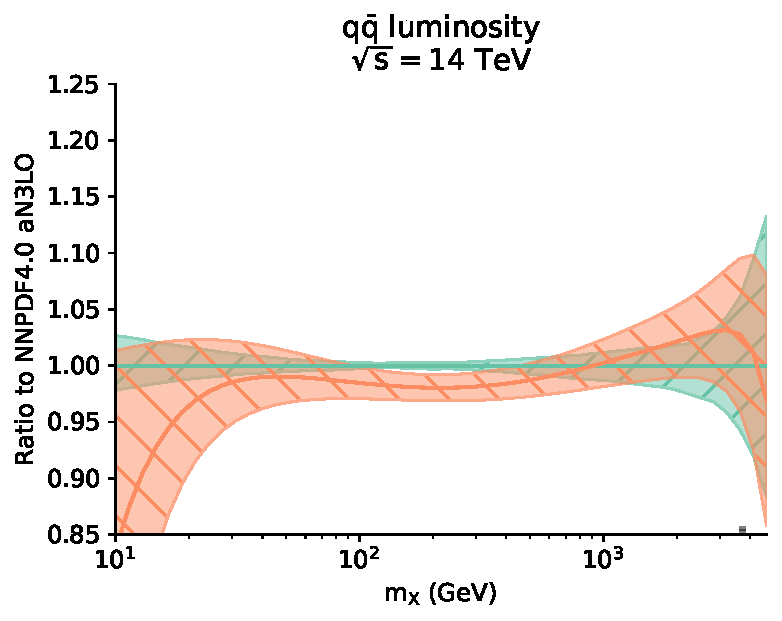
\includegraphics[width=0.45\textwidth]{figures/qqbar_plot_lumi1d_msht20.pdf}
%   \end{figure}
%   \begin{itemize}
%     \item Good agreement with MSHT20 for the quark luminosities
%     \item Also for gluon luminosities, except around the Higgs mass and high-mass
%     \item Similar data but different methodology (including splitting function parametrization)
%   \end{itemize}
% \end{frame}




\end{document}
